%!TEX root=../documentation-bachlorthesis-speicherarchitektur-lstucker.tex
\cleardoublepage
\chapter{Evaluation}

\section{Soll-Kriterien festlegen}
Die gewählten Kriterien für die Evaluation wurden zusammen mit dem Auftraggeber im Gespräch festgelegt. In einem weiteren Schritt wurden die einzelnen Kriterien nach ihrer logischen Zugehörigkeit hierarchisch geordnet und verfeinert (\refabb{abb:AHPKriterienbaum}). Die überarbeitete Kriterienauswahl wurde anlässlich eines weiteren Meetings mit dem Auftraggeber besprochen und fixiert. 

Die Kriterien sind für die späteren Verweise hierarchisch nummeriert.

\begin{center}
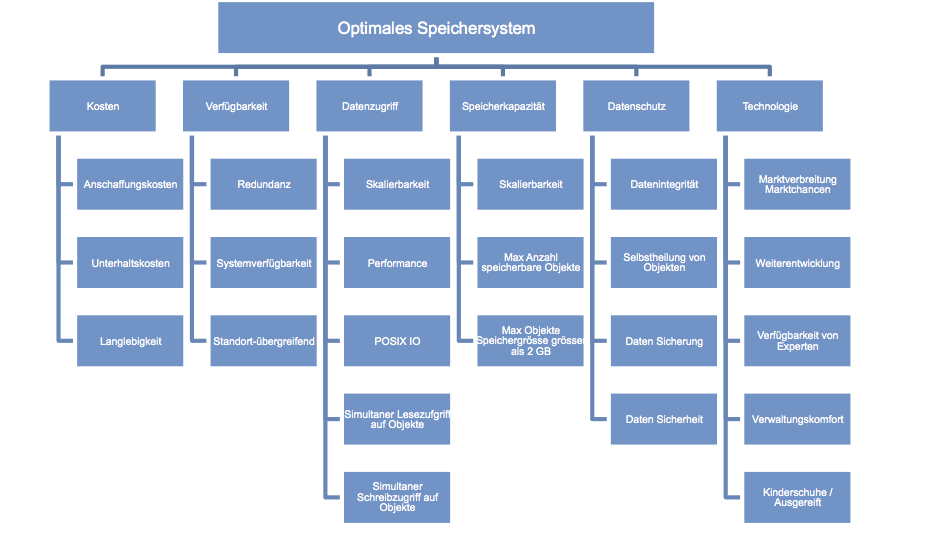
\includegraphics[width=\linewidth, keepaspectratio = true]{media/ahp_kriterienbaum.png}
\mycaption{figure}{\label{abb:AHPKriterienbaum} Optimales Speichersystem Kriterien}
\end{center}

\subsection{Haupt Soll-Kriterien festlegen}
Die Hauptkriterien sind in der obersten Hierarchie-Ebene dargestellt und werden durch ihre Unterkriterien weiter verfeinert und definiert.
\setcounter{paragraph}{0}
\renewcommand\theparagraph{Soll-\arabic{paragraph}}
\paragraph{Kosten}\label{Soll-1}
Die Kosten sollen einen gewinnbringenden Betrieb ermöglichen. 

\paragraph{Verfügbarkeit}\label{Soll-2}
Die Anforderungen an die Verfügbarkeit der Daten ist pro Szenario beschrieben und sollen entsprechend erfüllt werden. 

\paragraph{Datenzugriffe}\label{Soll-3}
Die Anzahl Datenzugriffe soll skalierbar sein. Es soll möglich sein, von mehreren Webservern gleichzeitig auf den Datenspeicher zugreifen zu können. Der Datenzugriff soll über POSIX IO oder über ein dokumentiertes API erfolgen können.

\paragraph{Speicherkapazität}\label{Soll-4}
Die Speicherkapazität soll die Speicheranforderungen der verschiedenen Szenerien erfüllen. Zudem soll die Speicherung von grossen Dateien bis zu 2 Gigabyte möglich sein.

\paragraph{Datenschutz}\label{Soll-5}
Der beschriebene Datenschutz soll jederzeit gewährleistet sein. Entscheidend ist der Schutz gegen die unerlaubte Veränderung von Daten. Für den Auftraggeber wichtig ist die laufende Sicherung der Daten, um den Verlust von Daten zu verhindern.

\paragraph{Technologie}\label{Soll-6}
Die Technologie bzw. das Produkt soll im Markt verbreitet sein, oder die Aussicht auf eine zukünftige Verbreitung im Markt. Zudem sollte die Technologie ausgereift sein, damit eine stabiler Betrieb gewährleistet ist. Nach Möglichkeit sollten genügen Experten verfügbar sein die sich mit der Technologie auskennen.

\subsection{Unter Soll-Kriterien festlegen}
Die Unterkriterien mit der gleichen Nummer-Ebene gehören zum selben Oberkriterium und werden später bei der Kriteriengewichtung untereinander direkt verglichen.

\setcounter{paragraph}{0}
\renewcommand\theparagraph{Soll-1-\arabic{paragraph}}

\paragraph{Anschaffungskosten}\label{Soll-1-1}
Die IT Infrastruktur soll über eine Abschreibungsdauer von 5 Jahren ausgelegt werden. Die gewählte Lösung kann sowohl eine Miete der Anlagen (Hosting) als auch die eigene Beschaffung der Hardware-Infrastruktur enthalten (managed servers). Um die Anbieter besser vergleichen zu können sind die Kosten auf 3 Jahre zu berechnen. 

\paragraph{Unterhaltskosten}\label{Soll-1-2}
Zu den Unterhaltskosten zählen sämtliche anfallenden Kosten für den Betrieb und Unterhalt der IT Infrastruktur eines Hosting-Anbieters. Nicht dazu zählen Kosten für die Anwendungs-Software (Anschaffung und Entwicklung) sowie die internen Kosten des Auftraggebers, sofern diese nicht direkt mit dem Betrieb der IT Infrastruktur verbunden sind (nicht direkt zurechenbare Kosten).

\paragraph{Nachhaltigkeit}\label{Soll-1-3}
Die Gesamtkosten (Anschaffung und Unterhalt) soll auf drei Jahre für alle Varianten gerechnet werden. Dabei soll auf eine gute Qualität der Komponenten für den Betrieb über 5 Jahre geachtet werden. Eine nachhaltige Planung steht im Vordergrund. Im Vergleich sollen sowohl die Anschaffungskosten und die Betriebskosten separat und auch insgesamt (TCO über 3 Jahre) verglichen werden.
Die Gesamtkosten sollten 50 \% der Einnahmen aus derselben Periode (3 Jahre) nicht übersteigen, damit ein langjähriger Betrieb wirtschaftlich realisierbar ist. Je tiefer die Gesamtkosten bei gleichbleibender Qualität, umso besser die Bewertung.

\setcounter{paragraph}{0}
\renewcommand\theparagraph{Soll-2-\arabic{paragraph}}

\paragraph{Redundanz}\label{Soll-2-1}
Die redundante Haltung von aktiven Daten, welche gelesen und manipuliert werden können, ermöglicht eine höhere Verfügbarkeit der Daten, z.B. beim Ausfall einer Systemkomponente. Die doppelte Datenhaltung wie sie bei der Datensicherung oder Archivierung entsteht, fällt nicht unter den Begriff "redundante Daten", da diese nicht direkt zur Erhöhung der Datenverfügbarkeit beiträgt. Die Speicherlösung sollte die Daten mindestens doppelt, oder wenn möglich dreifach redundant halten. 


\paragraph{Systemverfügbarkeit}\label{Soll-2-2}
Die verbesserte Systemverfügbarkeit, wird durch Software- oder Hardware-Redundanz erreicht. Die IT Infrastruktur (Server, Speicher, Netzwerk usw. soll möglichst redundant ausgelegt sein, um eine Verfügbarkeit nach AEC-3 Standard zu gewährleisten.

\paragraph{Standort-übergreifend}\label{Soll-2-3}
Die aktiven Daten sollen nach Möglichkeit an mindesten zwei voneinander getrennten Standorten gespeichert werden, um den Dienst auch im Falle des Ausfalls eines Rechenzentrums aufrecht erhalten zu können.

\setcounter{paragraph}{0}
\renewcommand\theparagraph{Soll-3-\arabic{paragraph}}

\paragraph{Skalierbarkeit}\label{Soll-3-1}
Die Speicherlösung sollte bei Bedarf den Speicher gleichzeitig an bis zu 30 Serversysteme zur Verfügung stellen können.

\paragraph{Performance}\label{Soll-3-2}
Die Speicherlösung soll eine IO-Performance von mindesten 27.31 MBit pro Sekunde haben.

\paragraph{POSIX IO}\label{Soll-3-3}
Die POSIX IO (inoffizielle Bezeichnung) ist ein Teil des POSIX Standards, welche die IO Schnittstelle für POSIX kompatible Applikationen definiert. Der Standard definiert ferner die Funktionen read(), write(), open(), close() inklusive deren Fehlerbehandlung. Die Speicherlösung soll für eine einfache Implementierung nach Möglichkeit diesen Standard unterstützen. 

\paragraph{Simultaner Lesezugriff auf Objekte}\label{Soll-3-4}
Das gleichzeitige Lesen desselben Objektes von zwei oder mehreren Serversystemen soll möglich sein.

\paragraph{Simulataner Schreibzugriff auf Objekte}\label{Soll-3-5}
Das gleichzeitige Schreiben auf dasselbe Objekte von zwei oder mehreren Serversystemen soll optional möglich sein.

\setcounter{paragraph}{0}
\renewcommand\theparagraph{Soll-4-\arabic{paragraph}}

\paragraph{Skalierbarkeit}\label{Soll-4-1}

\paragraph{Max Anzahl speicherbare Objekte}\label{Soll-4-2}
Das Speicherlösung soll die Anzahl der speicherbaren Objekte gemäss den Soll-Szenarien unterstützen. 

\paragraph{Max Objektgrösse von bis zu 2 GB}\label{Soll-4-3}
Das Speichersystem muss die Speicherung von Objekten mit einer Speichergrösse von bis zu 2 Gigabyte unterstützen.

\setcounter{paragraph}{0}
\renewcommand\theparagraph{Soll-5-\arabic{paragraph}}

\paragraph{Datenintegrität}\label{Soll-5-1}
Die Datenintegrität der gespeicherten Daten soll gewährleistet sein.

\paragraph{Selbstheilung von Objekten}\label{Soll-5-2}
Die Selbstheilung von beschädigten Daten soll nach Möglichkeit unterstützt werden. Diese Funktion ist bei der Verwaltung von grossen Datenmengen eine wichtige und geschätzte Funktion.

\paragraph{Datensicherung}\label{Soll-5-3}
Die gespeicherten Daten sollen mit einem effizienten Sicherungsverfahren gesichert werden können. Wenn die aktiven Daten nicht an zwei Standorten zur Verfügung gestellt werden können, wie in (\refsoll{Soll-2-3}) definiert, ist es zwingend erforderlich, dass der Sicherungsdatenträger an einem zweiten, physisch getrennten Standort gelagert wird.

\paragraph{Datensicherheit}\label{Soll-5-4}
Die Datenzugriffsberechtigung wird in der Applikation implementiert. Die Speicherlösung soll zudem sicherstellen, dass die Daten nicht von unerlaubten Dritten gelesen oder manipuliert werden können (physischer und logischer Zugriffsschutz).

\setcounter{paragraph}{0}
\renewcommand\theparagraph{Soll-6-\arabic{paragraph}}

\paragraph{Marktverbreitung / Marktchancen}\label{Soll-6-1}
Die Speicherlösung soll im Markt etabliert sein oder Tendenzen aufweisen, welche in den nächsten fünf Jahren die Verbreiterung im Markt wahrscheinlich erscheinen lässt.

\paragraph{Weiterentwicklung}\label{Soll-6-2}
Die Speichertechnologien, welche aktiv weiterentwickelt werden, sollen höher bewertet werden.

\paragraph{Verfügbarkeit von Experten}\label{Soll-6-3}
Die Verfügbarkeit von Experten einer etablierten Speicherlösungstechnologie soll sichtbar sein. Dabei soll das Expertenwissen regional breit verfügbar sein. Die Verfügbarkeit von Experten in der Schweiz ist höher zu werten als im Ausland.

\paragraph{Verwaltungskomfort}\label{Soll-6-4}
Die Speichertechnologie soll für die geforderte Datenmengen mit einem möglichst geringem Verwaltungsaufwand ermöglichen.

\paragraph{Kinderschuhe / Ausgereift}\label{Soll-6-5}
Die Speichertechnologie soll ausgereift und stabil laufen. Eine Implementierung von Beta-Versionen ist nicht erwünscht.

\section{KO-Kriterien}
Die KO-Kriterien sind Muss-Kriterien, welche von dem gewählten Speichersystem erfüllt werden müssen. Speichersysteme welche die KO-Kriterien nicht erfüllen, werden bei der AHP-Evaluation ausgeschlossen. Die KO-Kriterien wurde mit dem Auftraggeber besprochen und vereinbart.

\setcounter{paragraph}{0}
\renewcommand\theparagraph{KO-\arabic{paragraph}}

\paragraph{Dateigrösse bis 2 Gigibyte}\label{KO-1}
Die Speicherung von Dateien muss eine Objektgrösse von bis zu 2 Gibibyte erlauben.

\paragraph{Speicherkapazität Szenarien}\label{KO-2}
Die geforderten Speicherkapazitäten der Szenerien plus dem benötigten Speicherplatz für die Datenredundanz muss von der Speicherlösung unterstützt werden.

\paragraph{Kosten-Spannweite}\label{KO-3}
Die Kosten der teuersten Speicherlösung, darf nicht dreimal teurer sein, als die günstigste Lösung.

\section{Auswahl der Alternativen / Vertreter}
Mit dem Auftraggeber wurde definiert, dass für die Speicherlösungen, SAN, NAS, Distributed Filesystem Cluster, Online Speicher und dedizierter Webserver je ein Vertreter für die Evaluation ausgewählt werden sollen. Die Lösungen wurden nach Marktverbreitung und Technologie-Leader ausgewählt.

Die Alternativen/ Vertreter sind für die späteren Verweise nummeriert.

\setcounter{paragraph}{0}
\renewcommand\theparagraph{Al-\arabic{paragraph}}
\paragraph{Hetzner}\label{Al-1}
Dedizierte Webserver zählen im engeren Sinn nicht als reine Speicherlösungen. Der deutsche Hosting-Anbieter Hetzner bietet allerdings dedizierte Webserver mit der in Szenario 1 geforderten Speicherkapazität (siehe \refsec{Szenario-1}). Die bestehende Lösung wurde mit Hetzner Webserver realisiert. Hetzner als dedizierter Webserver Anbieter wurde deshalb auch berücksichtigt. 

\paragraph{NetApp NFS}\label{Al-2}
Als Vertreter für die NAS Speicherlösung wurde die NetApp FAS2240-4 gewählt. Für die Entscheidung zu NetApp haben dazu beigetragen, dass die Firma NetApp zu den Marktführern im NAS Bereich gehört und von Gartner als innovativ eingestuft wurde. Zudem pflegt die Firma ein breites Partnernetzwerk in der Schweiz.

\paragraph{NetApp iSCSI}\label{Al-3}
Als Vertreter für Block Speicherlösung wurde ebenfalls die NetApp FAS2240-4 gewählt. Die NetApp FAS2240-4 beherrscht ebenfalls iSCSI und FC SAN und kann somit als Block Speicherlösung ebenfalls eingesetzt werden. Für iSCSI im Vergleich zu FC-SAN spricht, dass neben der Ethernet-Netzwerk Technologie nicht zusätzliche Netzwerk Technologien eingesetzt werden müssen.

\paragraph{OpenStack Object Storage}\label{Al-4}

Als Vertreter für verteilten Speicher war ursprünglich Hadoop HDFS vorgesehen. In der aktuellen Version ist der Name-Node von HDFS noch ein Single Point of Failure (SPOF). Zudem liegen die Stärken bei HDFS bei den Datenprozessen für gespeicherte Objekte mittels MapReduce Algorithmus. Aus diesem Grund wurden weitere verteilte Dateisystem untersucht, wie etwa GlusterFS und OpenStack Object Storage. OpenStack Object Storage soll von der Architektur vergleichbar sein wie Amazon S3. Bei gewichtigen Online Speicheranbieter wird RackSpace erfolgreich eingesetzt. Ein weiterer Grund die für OpenStack Object Storage spricht, ist das gelungene quelloffene Projekt, das viele namhafte IT-Hersteller als Partner gewinnen konnte.

\paragraph{Amazon S3}\label{Al-5}
Amazon S3 wurde als Representant für Online Speicherlösungen gewählt. Amazon S3 ist gemäss \refsec{sec:MarktEtabliert} einer der etabliertesten Anbieter, wenn nicht die erfolgreichste Online Speicherlösung zur Zeit. Amazon betreibt mehrere Rechenzentrum verteilt auf mehrere Kontinenten. Für den Auftraggeber würde das Europäische Rechenzentrum in Frage kommen.


\subsection{Gewichtung der Soll-Kriterien mit AHP}

In diesem Abschnitt werden alle Soll-Kriteren der gleichen Hierarchie-Ebene bzw. gleichen Unter-Kriterien paarweise miteinander verglichen und mit der Skala \reftab{tab:9PBewertungsskala} aus dem \refchap{kab:Entscheidungsfindung} gewichtet.

% Vergleich mit Kosten
\paragraph*{\refsoll{Soll-1} verglichen mit \refsoll{Soll-2} (\ref{Soll-1}/\ref{Soll-2})} 
Mit steigenden Anforderungen an die Verfügbarkeit steigen auch die Kosten. Der Betrieb einer Infrastruktur eines Service-Anbieters muss kostendeckend sein. Einen Ausfall des Systems während definierten Betriebszeiten (das System muss online verfügbar sein), hat ebenfalls Auswirkungen auf das Unternehmen. So kann es zum Imageverlust, zu Kundenabgängen führen, oder die Zahlung von Entschädigungen erfordern. Die Rekonstruktion eines Datenverlustes kann trotz Sicherungskopie bei grossen Datenmengen zeitintensiv und kostspielig sein. Aus diesen Gründen ist ein gute Balance zwischen Kosten und Verfügbarkeit zu finden. Die Kosten sind deshalb im Vergleich zur Verfügbarkeit etwas grösser zu gewichten.

\textbf{Gewichtung: 3}

\paragraph*{\refsoll{Soll-1} verglichen mit \refsoll{Soll-3} (\ref{Soll-1}/\ref{Soll-3})}
Die Unterkriterien von Datenzugriffe sind mit der Skalierbarkeit der Datenzugriffe, Performance usw. wichtige Entscheidungskriteren. Dennoch sind diese im Vergleich zu den Kostenkriterien etwas tiefer zu gewichten. Grund dafür ist, dass der profitable Betrieb der Web-Applikation sichergestellt werden muss. Die Kosten sind deshalb etwas höher zu gewichten als die Datenzugriffe.

\textbf{Gewichtung: 3}

\paragraph*{\refsoll{Soll-1} verglichen mit \refsoll{Soll-4}}
Die Kosten und die Speicherkapazität sind gleich hoch bis etwas höher zu gewichten. Grund dafür ist, dass die Speicherlösung den rentablen Betrieb der Web-Applikation ermöglichen muss. Zugleich ist sicherzustellen, dass die geforderte Speicherkapazität vom Speichersystem erfüllt wird. Diese Kriterien sind deshalb gleich hoch zu gewichten.

\textbf{Gewichtung: 2}

\paragraph*{\refsoll{Soll-1} verglichen mit \refsoll{Soll-5}}
Für eine Web-Dienstleistung ist der Schutz der Daten wichtig. Wird die Plattform Opfer eines Hackersangriffes und wird dies publik, kann dies zu einem grossen Imageverlust führen. Aus diesem Grund ist sicherzustellen, das die Web-Applikation sicher betrieben werden kann. Die Sicherheit muss jedoch in erster Linie auf der Web-Applikation und dem Webserver sichergestellt werden und in zweiter Priorität auf dem Speichersystem. Die Kosten sind deshalb im Vergleich zum Datenschutz sehr viel bis absolut höher zu gewichten.

\textbf{Gewichtung: 8}

\paragraph*{\refsoll{Soll-1} verglichen mit \refsoll{Soll-6}}
Wie in den anderen Vergleichen ist sicherzustellen, dass die Web-Applikation rentabel betrieben werden kann. Deshalb sind möglichst tiefe Betriebskosten anzustreben. Die Kosten sind deshalb in Vergleich zur Technologie erheblich grösser zu gewichten.

\textbf{Gewichtung: 7}

% Vergleich mit Verfügbarkeit
\paragraph*{\refsoll{Soll-2} verglichen mit \refsoll{Soll-3}}
Aus Sicht des Anwenders ist die Verfügbarkeit der Daten höher zu gewichten als der möglichst schnelle Zugriff oder die Art und Weise wie der Zugriff stattfindet. Allerdings kann eine lange Wartezeit beim Ausliefern der Daten für den Anwender ebenfalls als "'nicht verfügbar"' empfunden werden. Es ist daher wichtig, dass der Zugriff auch vom Speichersystem effizient bewältig werden kann. Die Verfügbarkeit ist deshalb gleich bis etwas grösser zu gewichten als der Datenzugriff.

\textbf{Gewichtung: 2}

\paragraph*{\refsoll{Soll-2} verglichen mit \refsoll{Soll-4}}
Zum Geschäftsmodell der Web-Applikation gehört das Bereitstellung von Speicherkapazität für die Speicherung von grossen Bilddaten. Sind die Speicherkapazitäten ausgeschöpft und ist keine Wachstum mehr in der Speicherkapazität möglich, verliert der Auftraggeber ein neues Geschäft oder verliert gar einen bestehenden Kunden und kann mit dem Marktwachstum nicht Schritt halten. Aus diesem Grund ist die Verfügbarkeit etwas geringer zu gewichten als die Speicherkapazität.

\textbf{Gewichtung: 1/3}

\paragraph*{\refsoll{Soll-2} verglichen mit \refsoll{Soll-5}}
Um eine möglichst hohe Verfügbarkeit zu erreichen, werden zur Gewährleistung der Verfügbarkeit Massnahmen für den Datenschutz unternommen. Aus diesem Grund ist die Verfügbarkeit höher zu gewichten. 
Die Verfügbarkeit kann auch durch Schwachstellen erheblich höher zu gewichten sein als der Datenschutz.

\textbf{Gewichtung: 5}

\paragraph*{\refsoll{Soll-2} verglichen mit \refsoll{Soll-6}}
Für den Betrieb ist sicherzustellen, dass die Verfügbarkeit gewährleistet ist. Im Vergleich zur Marktverbreitung und die Verfügbarkeit von Experten ist deshalb die Verfügbarkeit erheblich bis sehr viel grösser zu gewichten.

\textbf{Gewichtung: 6}

% Vergleich mit Datenzugriffe
\paragraph*{\refsoll{Soll-3} verglichen mit \refsoll{Soll-4}}
Die Skalierbarkeit der Datenzugriff ist für ein Speichersystem fast gleich wichtig wie die Skalierbarkeit der Speicherkapazität. Die Art und Weise wie der Zugriff stattfindet, ist hingegen weniger wichtig als die maximale Grösse eines Objektes. Deshalb ist der Datenzugriff etwas weniger gross zu gewichten als die Speicherkapazität. 

\textbf{Gewichtung: 3}

\paragraph*{\refsoll{Soll-3} verglichen mit \refsoll{Soll-5}}
Für die Web-Applikation ist es wichtig, dass die geforderten Zugriffe auf das Speichersystem verarbeitbar sind. Die Sicherheit der Daten soll zudem vorwiegend aus Sicht der Applikation sichergestellt werden. Aus diesem Grund ist der Datenzugriff sehr viel grösser zu gewichten als der Datenschutz.

\textbf{Gewichtung: 7}

\paragraph*{\refsoll{Soll-3} verglichen mit \refsoll{Soll-6}}
Für die Web-Applikation ist es wichtig, dass die geforderten Zugriffe auf das Speichersystem verarbeitbar sind. Für den Langzeitbetrieb ist es aber auch wichtig, dass die Speichertechnologie mit den künftîgen Anforderungen des Marktes Schritt halten kann. Deshalb ist der Datenzugriff erheblich grösser zu gewichten als die Technologie.

\textbf{Gewichtung: 5}

% Vergleich mit Speicherkapazität
\paragraph*{\refsoll{Soll-4} verglichen mit \refsoll{Soll-5}}
Zum Geschäftsmodell der Web-Applikation gehört das Bereitstellung von Speicherkapazität zur Speicherung von grossen Bilddaten. Sind die Speicherkapazitäten erschöpft und ist kein Wachstum mehr möglich, kann der Auftraggeber mit den Marktanorderungen nicht mehr Schritt halten. Der Datenschutz der Daten ist ebenfalls wichtig. Der Schutz der Daten muss jedoch hauptsächlich auf der Applikationsseite erfolgen. Aus diesem Grund ist die Speicherkapazität sehr viel bis absolut grösser zu gewichten als der Datenschutz.

\textbf{Gewichtung: 8}

\paragraph*{\refsoll{Soll-4} verglichen mit \refsoll{Soll-6}}
Für den langfristigen Betrieb ist es wichtig, dass die Technologie laufend den neuen Marktanforderungen angepasst werden kann und genügend Experten vorhanden sind, welche mit der Technologie vertraut sind. Für das Geschäftsmodell ist es aber wichtiger, die notwendige Speicherkapazität zur Verfügung stellen zu können. Deshalb ist die Speicherkapazität sehr viel wichtiger als die Technologie.

\textbf{Gewichtung: 7}

% Vergleich mit Datenschutz
\paragraph*{\refsoll{Soll-5} verglichen mit \refsoll{Soll-6}}
Für den langfristigen Betrieb ist es wichtig, dass die Technologie laufend den neuen Marktanforderungen angepasst werden kann und genügend Experten vorhanden sind, welche mit der Technologie vertraut sind. Aus diesem Grund ist der Datenschutz etwas bis erheblich geringer zu gewichten als die Technologie.

\textbf{Gewichtung: 4}

\begin{table}[htbp]
\caption{AHP Gewichtung Top Kriterien}
\begin{tabular}{|l|r|r|r|r|r|r|r|}
\hline
\multicolumn{ 8}{|c|}{\textbf{Top Kriterien}} \\ \hline
 & \multicolumn{1}{l|}{\textbf{K}} & \multicolumn{1}{l|}{\textbf{V}} & \multicolumn{1}{l|}{\textbf{D}} & \multicolumn{1}{l|}{\textbf{S}} & \multicolumn{1}{l|}{\textbf{Ds}} & \multicolumn{1}{l|}{\textbf{T}} & \multicolumn{1}{l|}{\textbf{Gewicht}} \\ \hline
\textbf{Kosten (K)} & \textbf{1} & 3 & 3 & 2 & 8 & 7 & 0.353 \\ \hline
\textbf{Verfügbarkeit (V)} & 1/3 & \textbf{1} & 2 & 1/3 & 5 & 6 & 0.155 \\ \hline
\textbf{Datenzugriff (D)} & 1/3 & 1/2 & \textbf{1} & 1/4 & 7 & 5 & 0.122 \\ \hline
\textbf{Speicherkapazität (S)} & 0.5 & 3 & 4 & \textbf{1} & 8 & 7 & 0.299 \\ \hline
\textbf{Datenschutz (Ds)} & 1/8 & 1/5 & 1/7 & 1/8 & \textbf{1} & 1/4 & 0.026 \\ \hline
\textbf{Technologie (T)} & 1/7 & 1/6 & 1/5 & 1/7 & 4 & \textbf{1} & 0.045 \\ \hline
\textbf{Konsistenz Kennzahl} & 0.083 \\ \cline{1-2}
\end{tabular}
\label{AHPTop}
\end{table}

\subsubsection*{Gewichtung Kosten}

Wie nach der Gewichtung und in der \reftab{tab:AHPKosten} zu entnehmen ist, haben die Unterhaltskosten, gefolgt von Langlebigkeit die höhere Gewichtung als die Anschaffungskosten.

Die Paarvergleiche im Detail:

\paragraph*{\refsoll{Soll-1-1} verglichen mit \refsoll{Soll-1-2} (\ref{Soll-1-1}/\ref{Soll-1-2})}
Die Betriebskosten sind der Hauptkostenfakor in der Lebenszeit eines Informations-Systems. Gemäss Gartner fielen die weltweiten IT-Kosten im Jahr 2011 um 20 \% für Computer Hardware und um 43 \% für IT-Serviceleistungen. Zudem steigen die Kosten zum Beispiel von Disk Array Speicher nach Ablauf der ordentlichen vom Hersteller gewährleisteten Wartung, wegen teuren weiterführenden Wartungsverträge stark an.
Aus diesem Grund sind die Anschaffungskosten im Vergleich zu den Unterhaltskosten erheblich geringer zu gewichten.

\textbf{Gewichtung: 1/5}

\paragraph*{\refsoll{Soll-1-1} verglichen mit \refsoll{Soll-1-3} (\ref{Soll-1-1}/\ref{Soll-1-3})}
Fällt die Langlebigkeit eines Systems, weil es technologisch veraltet ist oder weil die Kosten für Wartungsverträge nach Ablauf der ordentlichen Wartung im Vergleich zur Neubeschaffung unrentabel sind, kurz aus. Sind erneut Kosten in der Anschaffung und Migration der Daten notwendig. Aus diesem Grund sind die Anschaffungskosten im Vergleich zur Langlebigkeit etwas geringer zu gewichten.

\textbf{Gewichtung: 1/3}


\paragraph*{\refsoll{Soll-1-2} verglichen mit \refsoll{Soll-1-3} (\ref{Soll-1-2}/\ref{Soll-1-3})}
Der Hauptkostenfakor in der Lebenzeit eines Informationssystems sind die Betriebskosten. Steigen diese Kosten aufgrund hoher Wartungvertragskosten mit der Lebenspanne des Systems an, kann sich der Betrieb als unrentabel herausstellen. Aus diesem Grund sind die Betriebskosten im Vergleich zur Langlebigkeit etwas grösser zu gewichten.

\textbf{Gewichtung: 3}

\begin{table}[htbp]
\caption{AHP Kosten}
\begin{tabular}{|l|r|l|l|l|}
\hline
\multicolumn{ 5}{|c|}{\textbf{Kosten}} \\ \hline
 & \multicolumn{1}{l|}{\textbf{A}} & \textbf{U} & \textbf{L} & \textbf{Gewicht} \\ \hline
\textbf{Anschaffung (A)} & 1 & \multicolumn{1}{r|}{0,2} & \multicolumn{1}{r|}{0,333} & \multicolumn{1}{r|}{0,105} \\ \hline
\textbf{Unterhaltskosten (U)} & 5 & \multicolumn{1}{r|}{1} & \multicolumn{1}{r|}{3} & \multicolumn{1}{r|}{0,637} \\ \hline
\textbf{Langlebigkeit (L)} & 3 & \multicolumn{1}{r|}{0,333} & \multicolumn{1}{r|}{1} & \multicolumn{1}{r|}{0.258} \\ \hline
\textbf{Konsistenz Kennzahl} & 0.033 \\ \cline{1-2}
\end{tabular}
\label{tab:AHPKosten}
\end{table}

\subsubsection*{Gewichtung Verfügbarkeit}

Wie nach der Gewichtung und in der \reftab{tab:AHPVerfügbarkeit} zu entnehmen ist, hat die Redundanz eine erheblich höhere Gewichtung als die Systemverfügbarkeit und Standortübergreifende Verfügbarkeit.

Die Paarvergleiche im Detail:

\paragraph*{\refsoll{Soll-2-1} verglichen mit \refsoll{Soll-2-2} (\ref{Soll-2-1}/\ref{Soll-2-2})}
Die Daten eines Informationssystem sind dessen wertvollstes Gut. Mit höherer Redundanz der Daten steigt auch die Verfügbarkeit der Daten.
Die Gesamtverfügbarkeit hängt jedoch auch von der Verfügbarkeit der einzelnen Systemkomponenten zusammen. Deshalb sollten die Daten systemübergreifend redundant sein, um ein hohe Verfügbarkeit zu gewährleisten. Gemäss eigener Erfahrungen ist die Zahl der Datenträgerausfällen höher als die restlichen Komponentenausfällen eines Systems. Die Datenredundanz ist deshalb erheblich grösser zu gewichten als die Systemredundanz.

\textbf{Gewichtung: 5}

\paragraph*{\refsoll{Soll-2-1} verglichen mit \refsoll{Soll-2-3} (\ref{Soll-2-1}/\ref{Soll-2-3})}
Die Standortübergreifende Verfügbarkeit der Daten kann nur mit Redundanz der Daten erreicht werden. Aus diesem Grund ist die Datenredundanz absolut höher zu gewichten als die standortübergreifende Verfügbarkeit.

\textbf{Gewichtung: 9}

\paragraph*{\refsoll{Soll-2-2} verglichen mit \refsoll{Soll-2-3} (\ref{Soll-2-2}/\ref{Soll-2-3})}
Die standortübergreifende Verfügbarkeit des System kann, erreicht werden, wenn die Daten auf mehrere Standorte verteilt werden und an diesen Standorten die Daten von einem lokalen System gelesen werden können. Das zweite System sollte idealerweise ein baugleiches Gerät sein, welches am zweiten Standort abgeschaltet ist und bei einem Ausfall am Hauptstandort hochgefahren wird.
Um die Verfügbarkeit zu gewährleisten, sollten keine manuellen Eingriffe erforderlich sein, da diese mit einem Unterbruch der Dienstleistung verbunden wäre. Aus diesem Grund ist die Systemverfügbarkeit etwas höher bis erheblich höher zu gewichten als die standortübergreifende Verfügbarkeit.

\textbf{Gewichtung: 4}

\begin{table}[htbp]
\caption{AHP Verfügbarkeit}
\begin{tabular}{|l|c|c|c|l|}
\hline
\multicolumn{ 5}{|c|}{\textbf{Verfügbarkeit}} \\ \hline
 & \multicolumn{1}{l|}{\textbf{R}} & \multicolumn{1}{l|}{\textbf{Sv}} & \textbf{St} & \textbf{Gewicht} \\ \hline
\textbf{Redundanz (R)} & 1 & 5 & \multicolumn{1}{r|}{9} & \multicolumn{1}{r|}{0,743} \\ \hline
\textbf{Systemverfügbarkeit (Sv)} & 1/5 & 1 & \multicolumn{1}{r|}{4} & \multicolumn{1}{r|}{0,194} \\ \hline
\textbf{Standort-Übergreifend (St)} & 1/9 & 1/4 & \multicolumn{1}{r|}{1} & \multicolumn{1}{r|}{0,063} \\ \hline
\textbf{Konsistenz Kennzahl} & 0,061 \\ \cline{1-2}
\end{tabular}
\label{tab:AHPVerfügbarkeit}
\end{table}

\subsubsection*{Gewichtung Datenzugriff}

Wie nach der Gewichtung und in der \reftab{tab:AHPDatenzugriff} zu entnehmen ist, hat die Fähigkeit für simultane Lesezugriffe auf Objekte dicht gefolgt von Skalierbarkeit der Datenzugriffe die höchste Gewichtung, gefolgt von Performance und der Unterstützung von POSIX IO. Die kleinste Gewichtung hat der simultane Schreibzugriff auf Objekte.


Die Paarvergleiche im Detail:

\paragraph*{\refsoll{Soll-3-1} verglichen mit \refsoll{Soll-3-2} (\ref{Soll-3-1}/\ref{Soll-3-2})}
Die Skalierung der Anzahl Datenzugriffe von mehreren Systemen ermöglicht die Web-Applikation höher redundant zu betreiben und die Verarbeitung der Bilddaten auf mehrere Server zu verteilen. Der maximale Datendurchsatz ist daher weniger bedeutend als dessen balansierten Verteilung der Zugriffe auf mehrere Server. Eine Speicherlösung, welche eine schlechte Performance aufweist, skaliert in der Regel ebenfalls nicht. Aus diesem Grund ist die Skalierung der Datenzugriffe etwas grösser zu gewichten als die Performance 

\textbf{Gewichtung: 3}

\paragraph*{\refsoll{Soll-3-1} verglichen mit \refsoll{Soll-3-3} (\ref{Soll-3-1}/\ref{Soll-3-2})}
Ist ein Zugriff auf die Daten über POSIX IO möglich, fällt allenfalls die Anpassung der entwickelten Web-Applikation geringer aus, als wenn er auf die Daten per API zugreifen muss. Für den Betrieb der Web-Applikation ist die Skalierung der Anzahl Datenzugriffe sehr viel bis absolut bedeutender als die Methode des Datenzugriffs.

\textbf{Gewichtung: 8}


\paragraph*{\refsoll{Soll-3-1} verglichen mit \refsoll{Soll-3-4} (\ref{Soll-3-1}/\ref{Soll-3-4})}
Der simultane Lesezugriff auf ein Objekt ermöglicht ein Objekt von mehreren Servern gleichzeitig zu lesen und dem Anwender darzustellen. Wird dies nicht unterstützt, kann dem Benutzer die Bilddatei nicht dargestellt werden, wenn ein anderer Besucher dieselbe Bilddatei gerade betrachtet. Aus diesem Grund ist die Skalierung und der simultane Lesezugriff auf Objekte gleich bedeutend.

\textbf{Gewichtung: 1}


\paragraph*{\refsoll{Soll-3-1} verglichen mit \refsoll{Soll-3-5} (\ref{Soll-3-1}/\ref{Soll-3-5})}
Der simultane Schreibzugriff auf ein Objekt erlaubt ein Objekt gleichzeitig von zwei oder mehreren Systemen bearbeiten zu können. Die Web-Applikation des Auftraggeber führt jedoch keine Änderungen an einer original Bilddatei durch, sondern erstellt modifizierte Kopien. Aus diesem Grund ist der gleichzeitige Schreibzugriff auf ein Objekt absolut geringer zu gewichten als die Skalierung des Datenzugriffs.

\textbf{Gewichtung: 9}

\paragraph*{\refsoll{Soll-3-2} verglichen mit \refsoll{Soll-3-3} (\ref{Soll-3-2}/\ref{Soll-3-3})}
Für den Betrieb der Web-Applikation ist die Performance der Datenzugriffe erheblich bis sehr viel bedeutender als die Methode des Datenzugriffs.

\textbf{Gewichtung 6}

\paragraph*{\refsoll{Soll-3-2} verglichen mit \refsoll{Soll-3-4} (\ref{Soll-3-2}/\ref{Soll-3-4})}
Die Performance ist erheblich geringer bedeutend als der simultane Lesezugriff auf Objekte. Grund dafür ist, dass das gleiche Objekte von mehreren Web-Servern gelesen werden kann, um diese den Website Besuchern darstellen können 

\textbf{Gewichtung: 1/5}

\paragraph*{\refsoll{Soll-3-2} verglichen mit \refsoll{Soll-3-5} (\ref{Soll-3-2}/\ref{Soll-3-5})}
Weil keine Manipulationen an der original Bilddatei durchgeführt wird, ist die Performance des Datenzugriff erheblich höher zu gewichten als der simultane Schreibzugriff auf Objekte. 

\textbf{Gewichtung: 5}


\paragraph*{\refsoll{Soll-3-3} verglichen mit \refsoll{Soll-3-4} (\ref{Soll-3-3}/\ref{Soll-3-4})}
Die Zugriffsmethode der Web-Applikation kann bei Bedarf durch die Entwickler angepasst werden. Für den Betrieb der Web-Applikation ist daher die Zugriffsmethode auf die Bilddaten erheblich geringer bedeutend als der simultane Lesezugriff.

\textbf{Gewichtung: 1/5}


\paragraph*{\refsoll{Soll-3-3} verglichen mit \refsoll{Soll-3-5} (\ref{Soll-3-3}/\ref{Soll-3-5})}
Weil keine Änderungen an original Bilddateien durchgeführt werden, ist es für den Auftraggeber bedeutender, dass ein Zugriff über POSIX IO möglich ist.

\textbf{Gewichtung: 3}


\paragraph*{\refsoll{Soll-3-4} verglichen mit \refsoll{Soll-3-5} (\ref{Soll-3-4}/\ref{Soll-3-5})}
Die Webapplikation des Auftraggeber führt keine Änderungen an der original Bilddatei durch, was den simultanen Schreibzugriff auf Objekten für den Betrieb der Web-Applikation von geringer Bedeutung ist. Der simultane Lesezugriff auf Objekten muss für den Betrieb der Web-Applikation möglich sein, damit die Bilddaten in mehreren Websitzungen gleichzeitig dargestellt werden können. Deshalb ist der simultane Lesezugriff gegenüber dem simultanen Schreibzugriff absolut höher gewichtet.

\textbf{Gewichtung: 9}

\begin{table}[htbp]
\caption{AHP Gewichtung Datenzugriff}
\begin{tabular}{|l|c|c|c|c|c|l|}
\hline
\multicolumn{ 7}{|c|}{\textbf{Datenzugriff}} \\ \hline
 & \multicolumn{1}{l|}{\textbf{SK}} & \multicolumn{1}{l|}{\textbf{Pe}} & \multicolumn{1}{l|}{\textbf{POI}} & \multicolumn{1}{l|}{\textbf{L}} & \multicolumn{1}{l|}{\textbf{S}} & \multicolumn{1}{l|}{\textbf{Gewicht}} \\ \hline
\textbf{Skalierbarkeit (Sk)} & 1 & 3 & 8 & 1 & 9 & 0,364 \\ \hline
\textbf{Performance (Pe)} & 1/3 & 1 & 6 & 1/5 & 5 & 0,158 \\ \hline
\textbf{POSIX IO (POI)} & 1/8 & 1/6 & 1 & 1/5 & 3 & 0,056 \\ \hline
\textbf{Simultaner Lesezugriff auf Objekte (L)} & 1 & 5 & 5 & 1 & 9 & 0,392 \\ \hline
\textbf{Simultaner Schreibzugriff auf Objekte (S)} & 1/9 & 1/5 & 1/3 & 1/9 & 1 & 0,031 \\ \hline
\textbf{Konsistenz Kennzahl} & 0,08 \\ \cline{1-2}
\end{tabular}
\label{tab:AHPDatenzugriff}
\end{table}

\subsubsection*{Gewichtung Speicherkapazität}


Wie nach der Gewichtung und in der \reftab{tab:AHPSpeicherkapazität} zu entnehmen ist, hat die Skalierbarkeit zusammen mit der max. Anzahl speicherbarer Objekte die höchste Gewichtung. Die Möglichkeit zur Speicherung von Objekte grösser als 2 GiB hat die tiefste Gewichtung, da die mindest Speichergrösse von bis zu 2 GiB bereits als KO Kriterium \ref{KO-1} festgelegt wurde und es sich somit um ein optionales Kriterium handelt.

Die Paarvergleiche im Detail:

\paragraph*{\refsoll{Soll-4-1} verglichen mit \refsoll{Soll-4-2} (\ref{Soll-4-1}/\ref{Soll-4-2})}
Die Skalierung der Speicherkapazität ist gleich zu gewichten wie die maximale Anzahl speicherbarer Objekte. Beides sind limitierende Faktoren, die bei erreichen der Grenze die Speicherung von neuen Objekten verunmöglichen. Erreicht man die Grenze der speicherbaren Objekten, kann die vorhandene freie Speicherkapazität nicht für neue Objekte verwendet werden. Umgekehrt wenn die Speicherkapazität nicht ausgebaut werden kann, kann die freie Kapazität an speicherbaren Objekten nicht dazu verwendet werden, neue Objekte zu speichern.

\textbf{Gewichtung: 1}

\paragraph*{\refsoll{Soll-4-1} verglichen mit \refsoll{Soll-4-3} (\ref{Soll-4-1}/\ref{Soll-4-3})}
Die Skalierbarkeit der Speicherkapazität ist für den Betrieb sehr viel höher zu gewichten als die maximale Speichergrösse für Objekte grösser als 2 Gigibyte.

\textbf{Gewichtung: 7}

\paragraph*{\refsoll{Soll-4-2} verglichen mit \refsoll{Soll-4-3} (\ref{Soll-4-2}/\ref{Soll-4-3})}
Die maximale Anzahl speicherbarer Objekte ist für den Betrieb sehr viel höher zu gewichten als die maximale Speichergrösse für Objekte grösser als 2 Gigibyte.

\textbf{Gewichtung: 7}

\begin{table}[htbp]
\caption{AHP Gewichtung Speicherkapazität}
\begin{tabular}{|l|c|c|c|l|}
\hline
\multicolumn{ 5}{|c|}{\textbf{Speicherkapazität}} \\ \hline
 & \multicolumn{1}{l|}{\textbf{S}} & \textbf{A} & \textbf{O} & \textbf{Gewicht} \\ \hline
\textbf{Skalierbarkeit (S)} & 1 & \multicolumn{1}{r|}{1} & \multicolumn{1}{r|}{7} & \multicolumn{1}{r|}{0,467} \\ \hline
\textbf{Max Anzahl speicherbare Objekte (A)} & 1 & \multicolumn{1}{r|}{1} & \multicolumn{1}{r|}{7} & \multicolumn{1}{r|}{0,467} \\ \hline
\textbf{Max Objekt Speichergrösse grösser als 2 GiB (O)} & 1/7 & \multicolumn{1}{r|}{1/7} & \multicolumn{1}{r|}{1} & \multicolumn{1}{r|}{0.067} \\ \hline
\textbf{Konsistenz Kennzahl} & 0 \\ \cline{1-2}
\end{tabular}
\label{tab:AHPSpeicherkapazität}
\end{table}

\subsubsection*{Gewichtung Datenschutz}

Wie nach der Gewichtung und in der \reftab{tab:AHPDatenschutz} zu entnehmen ist, hat das Kriterium Datensicherung gefolgt von Datenintegrität die höchste Gewichtung. Erheblich weniger Gewichtung haben Selbstheilung von Objekten und Datensicherheit.

Die Paarvergleiche im Detail:


\paragraph*{\refsoll{Soll-5-1} verglichen mit \refsoll{Soll-5-2} (\ref{Soll-5-1}/\ref{Soll-5-2})}
Damit das Speichersystem beschädigte Objekte selbständig heilen kann, ist es erforderlich, dass die Objekte redundant gespeichert werden und die Integrität der gespeicherten Objekte geprüft wird. Die Integrität der Objekte wird dabei mit einer zuvor erstellten und gespeicherten Hash-Prüfsumme verglichen. Aus diesem Grund ist die Datenintegrität erheblich höher zu gewichten als die Selbstheilung von Objekten.

\textbf{Gewichtung: 5}

\paragraph*{\refsoll{Soll-5-1} verglichen mit \refsoll{Soll-5-3} (\ref{Soll-5-1}/\ref{Soll-5-3})}
Verliert man alle primären Daten durch einen Hard- bzw. Software Fehler oder durch unerlaubtes Einwirken von Dritten, ist es unerlässlich, dass eine vollständige und konsistente Sicherungskopie der Daten besteht, um keinen totalen Datenverlust hinnehmen zu müssen.
Wenn ferner die Datenintegrität nicht sichergestellt ist, besteht ebenfalls die Gefahr eines Datenverlustes. Ist ein Objekt nicht mehr integer sondern korrupt und wird dies nicht vor der Datensicherung festgestellt, besteht die Gefahr eines Datenverlustes.
Der Verlust aller Daten ist schwerwiegender als der Verlust einzelner Daten.
Aus diesem Grund ist die Datenintegrität geringer zu gewichten als die Datensicherung.

\textbf{Gewichtung: 1/3}

\paragraph*{\refsoll{Soll-5-1} verglichen mit \refsoll{Soll-5-4} (\ref{Soll-5-1}/\ref{Soll-5-4})}
Primär muss bei einer Webapplikation die Datensicherheit innerhalb der Webapplikation sichergestellt werden. Aus diesem Grund ist die Datensicherheit sehr viel höher zu gewichten als die Datenintegrität.

\textbf{Gewichtung: 7}

\paragraph*{\refsoll{Soll-5-2} verglichen mit \refsoll{Soll-5-3} (\ref{Soll-5-2}/\ref{Soll-5-3})}
Die Selbstheilung von Daten stellt sicher, dass alle redundant gespeicherten Primären-Daten integer sind. Durch die Selbstheilung verringert sich das Risiko des Datenverlustes. 
Der Verlust aller Daten ist jedoch schwerwiegender als der Verlust einzelner Daten.
Aus diesem Grund ist die Selbstheilung der Daten erheblich geringer zu gewichten als die Datensicherung.

\textbf{Gewichtung: 1/5}

\paragraph*{\refsoll{Soll-5-2} verglichen mit \refsoll{Soll-5-4} (\ref{Soll-5-2}/\ref{Soll-5-4})}
Primär muss bei einer Webapplikation die Datensicherheit innerhalb der Webapplikation sichergestellt werden. Aus diesem Grund ist die Selbsheilung der Daten etwas höher zu gewichten als die Datensicherheit.

\textbf{Gewichtung: 3}

\paragraph*{\refsoll{Soll-5-3} verglichen mit \refsoll{Soll-5-4} (\ref{Soll-5-3}/\ref{Soll-5-4})}
Die Datensicherheit ist primär auf der Web-Applikationschicht zu gewährleisten und zu realisieren. Erfährt man einen Datenverlust durch das Einwirken von Dritten, ist sicherzustellen, dass eine Sicherungskopie der Daten existiert. Aus diesem Grund ist die Sicherung der Daten sehr viel höher zu gewichten als die Sicherheit. 

\textbf{Gewichtung: 7}

\begin{table}[htbp]
\caption{AHP Gewichtung Datenschutz}
\begin{tabular}{|l|c|c|c|c|l|}
\hline
\multicolumn{6}{|c|}{\textbf{Datenschutz}} \\ \hline
 & \multicolumn{1}{c|}{\textbf{I}} & \multicolumn{1}{c|}{\textbf{H}} & \multicolumn{1}{c|}{\textbf{B}} & \multicolumn{1}{c|}{\textbf{S}} & \multicolumn{1}{l|}{\textbf{Gewicht}} \\ \hline
\textbf{Datenintegrität (I)} & 1 & 5 & 1/3 & 7 & \multicolumn{1}{r|}{0,311} \\ \hline
\textbf{Selbstheilung von Objekten (H)} & 1/5 & 1 & 1/5 & 3 & \multicolumn{1}{r|}{0,097} \\ \hline
\textbf{Datensicherung (B)} & 3 & 5 & 1 & 7 & \multicolumn{1}{r|}{0,544} \\ \hline
\textbf{Datensicherheit (S)} & 1/7 & 1/3 & 1/7 & 1 & \multicolumn{1}{r|}{0,048} \\ \hline
\textbf{Konsistenz Kennzahl} & 0,084 \\ \cline{1-2}
\end{tabular}
\label{tab:AHPDatenschutz}
\end{table}

\subsubsection*{Gewichtung Technologie}

Wie nach der Gewichtung und in der \reftab{tab:AHPTechnologie} zu entnehmen ist, hat das Kriterium Ausgereift mit Abstand die höchste Gewichtung. Die zweithöchste Gewichtung ist der Weiterentwicklung zugeordnet, gefolgt von der Verfügbarkeit von Experten und der Marktverbreitung/Marktchancen. Am wenigsten Gewicht wird dem Verwaltungskomfort zugeteilt.

Die Paarvergleiche im Detail:


\paragraph*{\refsoll{Soll-6-1} verglichen mit \refsoll{Soll-6-2} (\ref{Soll-6-1}/\ref{Soll-6-2})} Ein Technologie, die nicht mehr weiterentwickelt wird, hat trotzt einer allfälligen grossen Marktverbreitung über kurz oder lang keine Chancen und wird durch neuere und bessere Technologien aus dem Markt verdrängt. Beim Entscheid zu einer neuen Lösung ist es wichtig, dass man sich für ein Technologie entscheidet, welche noch nicht am Ende ihres Lebenszyklus angelangt ist. Aus diesem Grund ist die Marktverbreitung/Marktchance erheblich geringer zu gewichten als die Weiterentwicklung.

\textbf{Gewichtung: 1/5}


\paragraph*{\refsoll{Soll-6-1} verglichen mit \refsoll{Soll-6-3} (\ref{Soll-6-1}/\ref{Soll-6-3})}
Mit einer hohe Marktverbreitung ist in der Regeln die Verfügbarkeit von Experten ebenfalls gegeben. Aus diesem Grund ist die Marktverbreitung und die Verfügbarkeit von Experten gleich zu gewichten

\textbf{Gewichtung: 1}

\paragraph*{\refsoll{Soll-6-1} verglichen mit \refsoll{Soll-6-4} (\ref{Soll-6-1}/\ref{Soll-6-4})}
Ein Produkt welches hohen Verwaltungskomfort aufweist, jedoch wegen anderen Faktoren ein schlechte Marktverbreitung oder Marktchancen aufweist, ist für den langfristigen Betrieb eher ungeeignet. Die Marktverbreitung ist deshalb etwas höher zu gewichten als der Verwaltungskomfort.

\textbf{Gewichtung: 3}

\paragraph*{\refsoll{Soll-6-1} verglichen mit \refsoll{Soll-6-5} (\ref{Soll-6-1}/\ref{Soll-6-5})}
Für den Betrieb der Web-Applikation ist es wichtig, dass die Speicherlösung technisch und und im Alltagseinsatz ausgereift ist. Die Marktverbreitung ist deshalb absolut geringer zu gewichten als eine ausgereifte Speicherlösung.

\textbf{Gewichtung: 1/9}

\paragraph*{\refsoll{Soll-6-2} verglichen mit \refsoll{Soll-6-3} (\ref{Soll-6-2}/\ref{Soll-6-3})}
Eine Technologie, welche nicht mehr weiter entwickelt wird, lauft Gefahr, den Marktanforderungen bald nicht mehr zu genügen und könnte in der Folge von neuen Technologien ersetzt werden. Der Rückgang der Marktanteile der Technologie hat auch zur Folge, dass der Nachwuchs sich in den alten Technologien ebenfalls weiterbilden muss. Dies wiederum hat zur Folge, dass die Anzahl Experten mittelfristig ebenfalls abnimmt. Aus diesem Grund ist die Weiterentwicklung erheblich höher zu gewichten als die Verfügbarkeit von Experten.

\textbf{Gewichtung: 5}

\paragraph*{\refsoll{Soll-6-2} verglichen mit \refsoll{Soll-6-4} (\ref{Soll-6-2}/\ref{Soll-6-4})}

Die Weiterentwicklung ist für den Langzeitbetrieb wichtiger als der Verwaltungskomfort. Bestehende Schwächen im Verwaltungskomfort könnten in weiterentwickelten Versionen behoben oder verbessert sein. Die Weiterentwicklung wird deshalb für den Langzeitbetrieb sehr viel höher gewichtet als der Verwaltungskomfort.

\textbf{Gewichtung: 7}

\paragraph*{\refsoll{Soll-6-2} verglichen mit \refsoll{Soll-6-5} (\ref{Soll-6-2}/\ref{Soll-6-5})}
Für den Betrieb der Web-Applikation ist es wichtig, dass die Speicherlösung technisch und betrieblich ausgereift ist. Die Weiterentwicklung ist deshalb erheblich geringer zu gewichten als eine ausgereifte Speicherlösung.

\textbf{Gewichtung: 1/5}


\paragraph*{\refsoll{Soll-6-3} verglichen mit \refsoll{Soll-6-4} (\ref{Soll-6-3}/\ref{Soll-6-4})}
Bietet ein Speicherlösung einen hohen Verwaltungskomfort, kann die Verwaltung in der Regel schneller und von weniger gut geschultem Personal durchgeführt werden. Folglich verringert sich die Abhängigkeit zu Experten. Für die Konzeption, Inbetriebnahme, spätere Optimierung und Problemlösungen der Speicherinfrastruktur ist man in der Regel weiterhin auf das Wissen von Experten angewiesen. Aus diesem Grund ist es wichtig, dass der Zugriff auf Expertenwissen vorhanden ist. Die Verfügbarkeit von Experten ist deshalb, erheblich höher zu gewichten als der Verwaltungskomfort. 

\textbf{Gewichtung: 5}

\paragraph*{\refsoll{Soll-6-3} verglichen mit \refsoll{Soll-6-5} (\ref{Soll-6-3}/\ref{Soll-6-5})}
Für den Betrieb der Web-Applikation ist es wichtig, dass die Speicherlösung technisch und betrieblich ausgereift sind. Ein nicht ausgereiftes Produkt könnte massive Mängel ausweisen, die einen effizienten Betrieb gefährden würden, falls dies nicht gänzlich durch Experten kompensiert werden könnte. Die Verfügbarkeit von Experten ist deshalb sehr viel geringer zu gewichten als die ausgereifte Speicherlösung.

\textbf{Gewichtung: 1/7}

\paragraph*{\refsoll{Soll-6-4} verglichen mit \refsoll{Soll-6-4} (\ref{Soll-6-3}/\ref{Soll-6-5})}
Für den Betrieb der Web-Applikation ist es wichtig, dass die Speicherlösung technisch und betrieblich ausgereift ist. Der höchste Verwaltungskomfort bringt letztendlich nichts, wenn das Produkt Mängeln aufweist und den Betrieb gefährdet.

Der Verwaltungskomfort ist deshalb absolut geringer zu gewichten als die ausgereifte Speicherlösung.

\textbf{Gewichtung: 1/9}

\begin{table}[htbp]
\caption{AHP Gewichtung Technologie}
\begin{tabular}{|l|c|c|c|c|c|r|}
\hline
\multicolumn{ 7}{|c|}{\textbf{Technologie}} \\ \hline
 & \textbf{M} & \textbf{W} & \textbf{E} & \textbf{V} & \textbf{A} & \multicolumn{1}{l|}{\textbf{Gewicht}} \\ \hline
\textbf{Marktverbreitung/Marktchancen (M)} & 1 & 1/5 & 1 & 3 & 1/9 & 0.064 \\ \hline
\textbf{Weiterentwicklung (W)} & 5 & 1 & 5 & 7 & 1/5 & 0.238 \\ \hline
\textbf{Verfügbarkeit von Experten (E)} & 1 & 1/2 & 1 & 5 & 1/7 & 0.079 \\ \hline
\textbf{Verwaltungskomfort (V)} & 1/3 & 1/7 & 1/2 & 1 & 1/9 & 0.031 \\ \hline
\textbf{Ausgereift (A)} & 9 & 5 & 7 & 9 & 1 & 0.588 \\ \hline
\textbf{Konsistenz Kennzahl} & \multicolumn{1}{r|}{0.094} \\ \cline{1-2}
\end{tabular}
\label{tab:AHPTechnologie}
\end{table}


\section{Analyse Alternativen auf KO-Kriterien}

\section{Daten Sammeln}
\subsection{\ref{Al-1}: Hetzner Server}
Hetzner ist einer der grössten Hosting Anbieter in Deutschland und bietet seit 1997 für Unternehmen und Privatpersonen Hosting-Produkte an. In den vergangenen Jahren hat Hetzner von diversen Computer-Magazinen Auszeichnungen bekommen. Hetzner betreibt in Deutschland mehrere Rechenzentren die mehrfach redundant an das Internet angeschlossen sind.

Die \refabb{abb:Hetzner-Infrastruktur} zeigt den gemieteten Hetzner Server mit dem internen RAID Disk Speicher. In \refabb{abb:HetznerRaidSpeicher} wird die interne Architektur des RAID-Speichers mit den verschiedenen Speicherschichten dargestellt.

\begin{center}
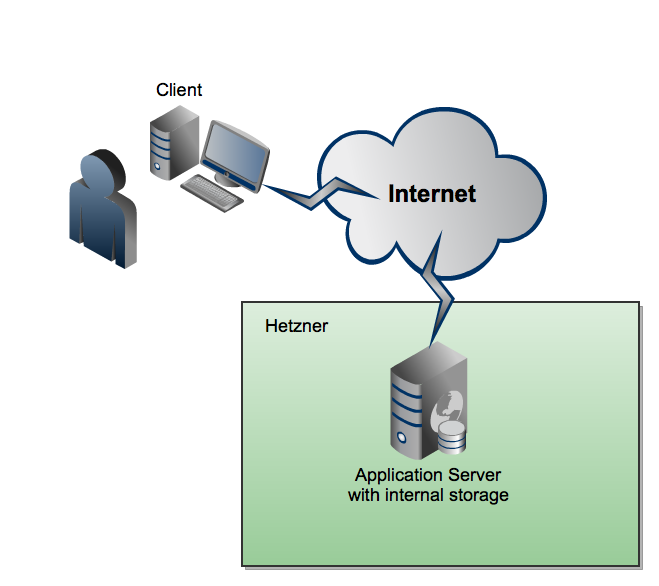
\includegraphics[width=\linewidth, keepaspectratio = true]{media/Hetzner.png}
\mycaption{figure}{\label{abb:Hetzner-Infrastruktur} Dezidierter Server System und Netzwerk Architektur }
\end{center}



\subsubsection*{Speicherkapazität}
Der grösste dedizierte Server, welcher Hetzner in seinem Produktkatalog führt, ist der Root-Server XS 29. Der XS 29 ist mit 15 mal 3 Terabyte SATA Festplatten ausgerüstet. Mit dem zusätzlich eingebauten Hardware-RAID-Controller lassen sich die 15 Festplatten zu einen RAID zusammenfügen.
Als CPU hat der Server einen Intel Xeon E3-1245 Quad-Core eingebaut und verfügt über 16 Gigabyte Hauptspeicher. 

Die max. Grösse einer Datei ist vom Dateisystem abhängig. ext3 oder "third extended filesystem" genannt, ist bei den meisten bekannten Linux Distributoren das standard Dateisystem. Die maximale Grösse einer Datei hängt von der verwendeten Blockgrösse ab. Nach eigenen Tests ist die standard Blockgrösse bei Debian, Ubuntu, Red Hat und Suse 4 Kibibyte gross. Bei einer Blockgrösse von 4 Kibibyte, kann eine Datei maximal 2 Tebibyte und das Dateisystem 16 Tebibyte gross sein. \cite{Card1993}

Die maximale Anzahl an Objekten hängt von der Grösse des Dateisystems ab. Bei einem 16 Tebibyte unterstützt die standard Konfiguration maximal 17'592'186'044'416 Objekte. 

\subsubsection*{Verfügbarkeit}
Die RAID-5 Konfiguration mit 15 Festplatten im RAID, bietet mit 38,192 Tebibyte gemäss \refeqlb{eqn:MaxSpeicherkapazitätHeztner} bei einfacher Redundanz die grösst mögliche Speicherkapazität. Wegen der möglicherweise langen Wiederherstellungs-Zeit (MTTR) dieser Konfiguration, ist man darauf angewiesen, dass der Ausfall vom eigenen Überwachungssystem erkannt und nach Benachrichtigung des Hetzner Support die defekte Festplatte rasch ausgetauscht wird. Die Festplatten selber sind während des Betriebs austauschbar, es ist somit kein Unterbruch des Betriebs erforderlich.

Der eingesetzte LSI RAID Kontrolle lässt auch die Konfiguration einer Hot-Spare Festplatte zu. Ein Host-Spare Festplatte ist ein leere ungenutzte Festplatte, die beim Ausfall einer Festplatte im RAID automatisch die defekte Festplatte ersetzt. 

Da es sich nur um ein Server System handelt, ist ein standortübergreifende Verfügbarkeit der Daten nicht möglich.


\begin{equation}
\mbox{Max Speicherkapazität} = (15 -1)* 2,728 \mathrm{\ TiB}= 38,192 \mathrm{\ TiB}
\label{eqn:MaxSpeicherkapazitätHeztner}
\end{equation}

\begin{equation}
\mbox{Max Speicherkapazität mit Hostspare} = (15 -1-1)* 2,728 \mathrm{\ TiB}= 35,464 \mathrm{\ TiB}
\label{eqn:MaxSpeicherkapazitätHeztnerHotspare}
\end{equation}

\subsubsection*{Datenzugriff}
Der Datenzugriff findet lokal über POSIX IO statt, dass heisst das die Web-Applikation auf dem selben Server betrieben wird. 

Der Lese- und Schreibzugriff ist auf den Server begrenzt. Theoretisch könnte der Speicher mit Protokollen wie NFS zwischen mehreren Systemen geteilt werden. Es handelt sich beim System um einen Miet-Server. Es kann deshalb nicht davon ausgegangen werden, dass weitere Miet-Server am selben Netzwerk-Knoten angeschlossen sind, oder sich sogar im gleichen Rechenzentrum befinden. Es muss aus diesen Gründen mit einer schlechten Bandbreite mit hoher Latenz zwischen den Systemen gerechnet werden, was die Teilung des Speichers aus Performancegründen unbefriedigend macht.

\begin{center}
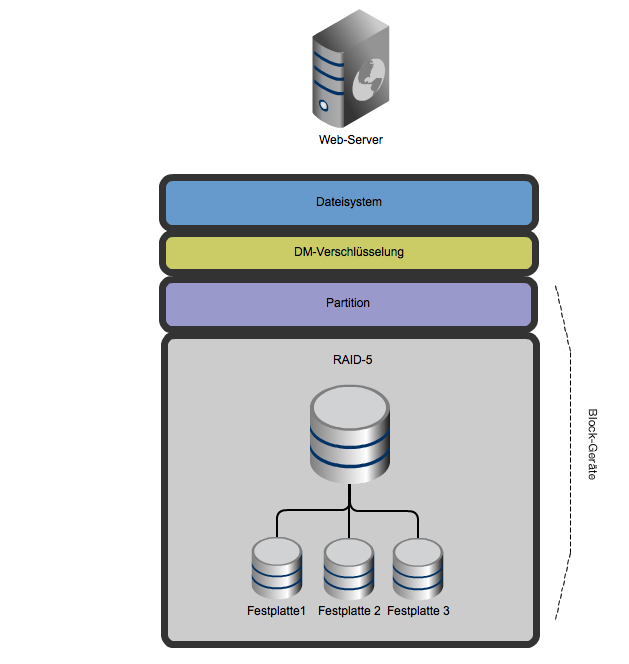
\includegraphics[width=\linewidth, keepaspectratio = true]{media/HetznerRAID.png}
\mycaption{figure}{\label{abb:HetznerRaidSpeicher} Interne Speicherarchitektur }
\end{center}

\subsubsection*{Datenschutz}
Die Integrität der Daten wird nur auf RAID Ebene sichergestellt und nicht auf Objekt-Ebene. Die Selbstheilung von Objekten wird nicht unterstützt.

Die Daten können mit einen RSYNC Job gesichert werden. Gegen eine zusätzliche Gebühre von 79 € für 10 GB ist die Datensicherung bei Hetzner möglich.

Der Datenzugriff lässt sich über die Dateiberechtigung im Dateisystem auf Benutzer- und Gruppen-Ebene steuern. Gegen den unerlaubten physischen Datenzugriff bietet die Verschlüsselung der Disk einen ausreichenden Schutz.

\subsubsection*{Technologie}
Die Konfiguration und Betrieb des Server inklusive RAID ist dem Mieter überlassen. Die RAID Technologie ist eine viel eingesetzte und bewährte Technologie.

Für die Konfiguration und den Betrieb des Servers reicht das Administratoren-Wissen für standard Linux aus.

Die Verwaltung des Speichers erfolgt über Kommandozeile bzw. über \gls{SSH}.

\subsubsection*{Kosten}
Abgesehen von den einmaligen Einrichtungskosten von 499 € und den Server Installationskosten gibt es keine weitere Investitionskosten. 

Für die Installation und Betrieb des gemieteten Servers ist der Mieter selber verantwortlich. Die Mietkosten betragen pro Monat 299 €.

Die Kosten für die Miete des Servers bleiben während der gesamten Mietdauer konstant. Die Kündigung ist jeweils auf 30 Tage zum Monatsende möglich. 

\paragraph*{Kosten Szenario-1}
Die Kosten für Szenario-1 betragen gemäss Zusammenstellung der Tabelle (10.9) Total € 11'163.00. Das entspricht zum aktuellen Tageskurs (13 April 2012) 13'422.95 CHF.

\begin{table}[htbp]
\caption{Kosten Hetzner Szenario-1}
\begin{small}
\begin{tabular}{|l|r|r|r|}
\hline
\textbf{Beschreibung} & \multicolumn{1}{l|}{\textbf{Kosten pro Stk/M.}} & \multicolumn{1}{l|}{\textbf{Anzahl}} & \multicolumn{1}{l|}{\textbf{Total}} \\ \hline
 \multicolumn{ 4}{c}{} \\ \hline
\multicolumn{ 4}{|c|}{\textbf{Investitionskosten}} \\ \hline
Einrichtung Root Server XS 29 & € 499.00 & 1 & € 499.00 \\ \hline \hline
 \multicolumn{ 3}{r|}{\textbf{Total:}} & \textbf{€ 499.00} \\ 
 \cline{4-4}
\multicolumn{ 4}{c}{} \\ \hline
\multicolumn{ 4}{|c|}{\textbf{Fortlaufende Kosten}} \\ \hline
Root Server XS 29 & € 299.00 & 1 & € 299.00 \\ \hline \hline
 \multicolumn{ 3}{r|}{\textbf{Total pro Monat:}} & € 299.00 \\
\cline{4-4}
 \multicolumn{ 3}{r|}{\textbf{Total 36 Monate:}} & \textbf{€ 10'764.00} \\ \cline{4-4}
 \multicolumn{ 4}{c}{} \\ \cline{4-4}
 \multicolumn{ 3}{r|}{\textbf{Total Gesamt:}} & \textbf{€ 11'163.00} \\ \cline{4-4}
\end{tabular}
\end{small}
\label{KostenHetznerS1}
\end{table}


\paragraph*{Kosten Szenario-2}
Es ist kein Produkt erhältlich, welches die Anforderungen der vorgeschlagenen Speicherkapazität von Szenario-2 erfüllen könnte.

\subsection{\ref{Al-2} und \ref{Al-3}: Netapp NFS und iSCSI}

Wie in der Markt Analyse erwähnt, ist NetApp der führende Anbieter im mittleren (engl. midrange) und oberen (Highend) Bereich von NAS und Speicherlösungen. Für beide Szenarien wurde das Modell FAS2240-4 gewählt. 

\begin{center}
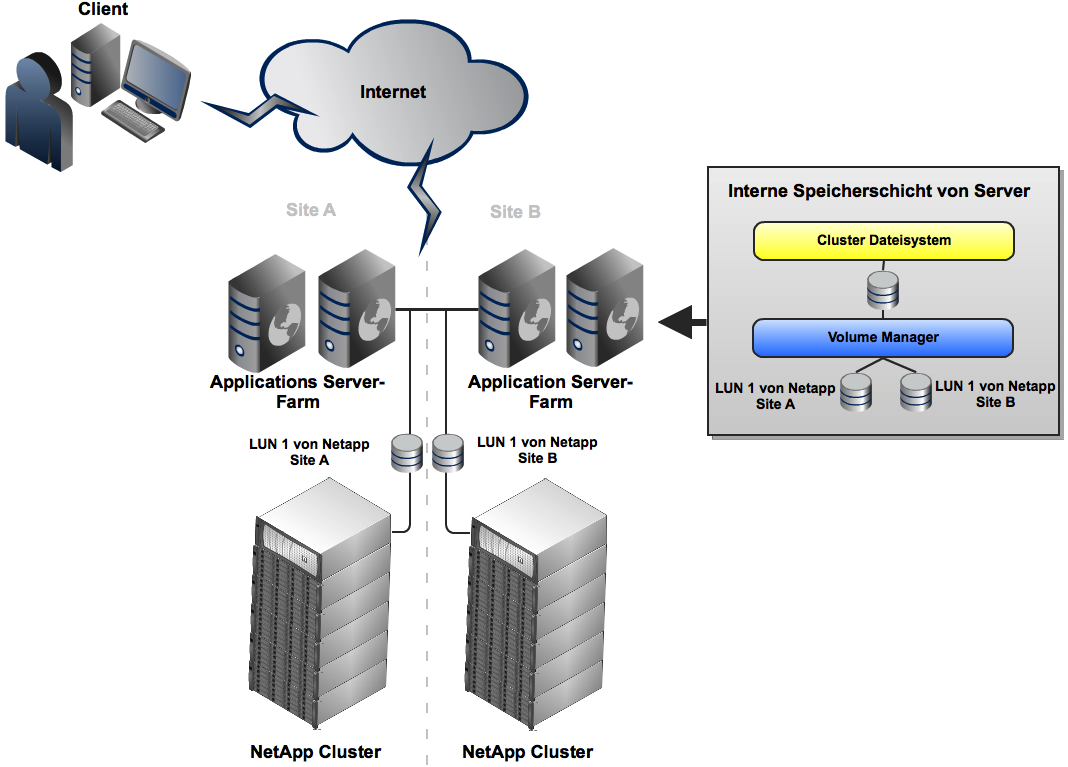
\includegraphics[width=\linewidth, keepaspectratio = true]{media/NetAppISCSI.png}
\mycaption{figure}{\label{abb:NetAppISCSI}NetApp iSCSI Architektur }
\end{center}


\subsubsection*{Verfügbarkeit}
Die Netapp hat mehrere Mechanismen für die Sicherstellung der Datenverfügbarkeit. So werden die Festplatten mittels RAID-DB System zusammen gefasst. RAID-DP ist eines auf Basis von RAID-4 von NetApp weiterentwickeltes RAID. Bei RAID-DP wird jedoch im Unterschied zu RAID-4 eine zusätzliche Paritäts-Festplatte eingesetzt. Wie in \refabb{abb:RAID-DP} ersichtlich, gibt es ein horizontale Parität und eine diagonale Parität. Die diagonale Parität ist durch die Farben dargestellt und auf der Festplatte DP gespeichert. Die horizontale Parität ist auf der Festplatte P gespeichert. Die mit D bezeichneten Festplatten sind normale RAID Daten-Festplatten. Die doppelte Parität hat den Vorteil, dass die Verfügbarkeit des RAID erhöht wird. So können bei einem RAID-DP gleichzeitig zwei Festplatten zur gleichen Zeit ausfallen, ohne dass dies zu einem Datenverlust führt, was in der Praxis immer wieder mal vorkommt. Im Vergleich dazu kann RAID-4 oder RAID-5 nur den Ausfall einer Festplatte kompensieren. \cite{White2010}

\begin{center}
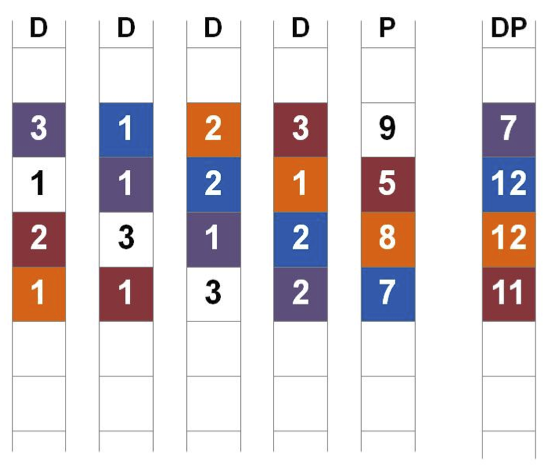
\includegraphics[ keepaspectratio = true]{media/raid-dp.png}
\mycaption{figure}{\label{abb:RAID-DP}NetApp RAID-DP doppelte Parität \cite{White2010}}
\end{center}

Als weitere Schutzmassnahme vor Datenverlusten empfiehlt NetApp den Einsatz von Spare-Festplatten. Durch den Einsatz von Spare-Festplatten kann die Wiederherstellungszeit MTTR verkleinert werden, da die Wiederherstellung automatisch starten kann. Die Anzahl an Spare-Festplatten ist abhängig von der Anzahl Festplatten und Enclosure.

Die NetApp FAS2240-4 ist mit zwei Storage Controller im Aktiv-/Aktiv-Betrieb mit Cluster Failover Funktion ausgerüstet.


\subsubsection*{Datenzugriff}
Der Datenzugriff auf die NetApp kann per NFS, CIFS, iSCSI oder Fibre Channel erfolgen.

Bei NFS ist es möglich, dass mehrere Server simultan eine Datei lesen. Das simultane Schreiben wird mit einem Sperr-Verfahren (engl. Locking) verhindert, damit die Dateikonsistenz gewährleistet bleibt.

Bei iSCSI wird der simultane Lesezugriff auf Dateien mittels clusterfähigem Dateisystem und Volume-Manager wie dem Global Filesystem bzw. LVM sichergestellt. Der simultane Schreibzugriff wird vom Dateisystem mit einem Sperrverfahren verhindert.

\begin{center}
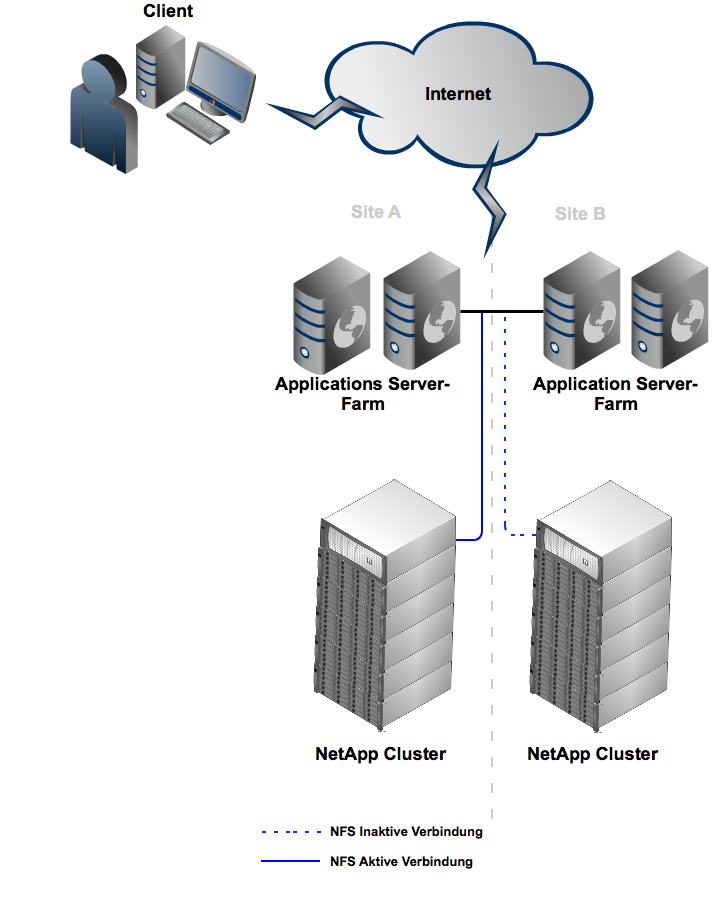
\includegraphics[width=\linewidth, keepaspectratio = true]{media/NetAppNFS.png}
\mycaption{figure}{\label{abb:NetAppNFS} NetApp NFS Architektur  }
\end{center}

\subsubsection*{Speicherkapazität}
Die maximale Grösse einer Datei bzw. eines Objekts wird bei NetApp durch die maximale Grösse des Aggregates bestimmt. Seit der Betriebsystem-Version OnTab 8.0 sind Aggregate von 100 TiB möglich.

Bei iSCSI werden auf der NetApp LUN Dateien erstellt, die über iSCSI anderen Servern zur Verfügung gestellt werden. Die LUN Datei ist für den zugeteilten Server wie eine gewöhnliche Disk. Die Limitierungen für die maximale Dateigrösse und maximale Anzahl an Dateien wird bei iSCSI nicht mehr durch die NetApp limitiert, sondern durch das auf dem Server verwendete Dateisystem. So gewährleistet Red Hat für Global Filesystem (GFS) maximal ein 100 Terabyte grosses Dateisystem produktiv zu betreiben. Dieselbe Einschränkung gilt für Dateien. 

Die Anzahl möglicher Objekte, die in einen NetApp Volumen gespeichert werden können, werden durch die Anzahl Inodes des WAFEL Dateisystem bestimmt. NetApp legt standardmässig für jedes 32KiB eine Inode an. Bei einen 100 TiB Volume können somit maximal 3'355'443'200 Objekte gespeichert werden (\refeql{eqn:MaxObjekteNetApp}).

\begin{equation}
\mbox{Max Objekte} = \frac{107'374'182'400 \mathrm{\ KiB}}{32 \mathrm{\ KiB}}= 3'355'443'200 
\label{eqn:MaxObjekteNetApp}
\end{equation}

Die maximale Anzahl möglicher Objekte eines GFS Dateisystem ist variable. Inodes werden dynamisch alloziert.

\subsubsection*{Datenschutz}
NetApp speichert die Daten auf die Disk in 4 Kilo Byte Blocks. Zu jedem 4 Kilo Byte Block berechnet NetApp ein Prüfsumme und speichert diese in die Block Metadaten. Wenn der Block zu einem späteren Zeitpunkt wieder gelesen wird, berechnet die NetApp die Prüfsumme erneut und vergleicht diese mit der gespeicherten Prüfsumme. Stimmt diese nicht überein, wird der Block mittels den Paritäts-Daten neu geschrieben, erneut gelesen und geprüft. Um die Integrität von Daten zu gewährleisten, auf welche über einen längeren Zeitraum nicht mehr zugegriffen wurde, wie dies zum Beispiel bei Archivdaten der Fall ist, bietet NetApp ein konfigurierbare RAID Funktion (engl. RAID scrub) zum Durchkämmen und Prüfen der Daten. Die Funktion kann zeitgesteuert durchgeführt werden oder wenn das System sich im Leerlauf befindet. \cite{Sundaram2006}

Zu beachten ist, dass die Prüfsumme auf dem Block nur auf der Speicherebene Wirkung hat. Fehler die in einer höheren Ebene entstanden sind, wie zum Beispiel beim Einsatz von iSCSI zusammen mit einen Dateisystem, könnte bereits ein Fehler im Dateisystem durch einen Softwarefehler oder Memoryfehler entstanden sein. 

NetApp bietet mehrere Möglichkeiten eine Sicherungskopie der Daten herzustellen. Beim Einsatz von NFS oder iSCSI können die Daten über die Web-Servern mit einer handelsüblichen Sicherungs-Software gesichert werden. Bei NFS wird dazu die angefügten NFS Freigaben gesichert, bei iSCSI werden die Daten wie bei allen anderen Dateisystemen gesichert. Zu beachten ist bei diesen Verfahren, dass die Daten von der NetApp über den Server transferiert werden müssen und dadurch der Web-Server mit der Sicherungsaufgabe belastet wird. Neben der Sicherung der NetApp über den Server lässt sich die NetApp auch direkt sichern. Diese erfolgt mittels Network Data Management Protocol (NDMP) oder Mittels Snapshots. 

NDMP ist eines von NetApp mitentwickeltes Protokoll, welches für die Sicherung von NAS Geräte entwickelt wurde. Das Problem bei NAS Geräte ist, dass auf ihnen ein dediziertes Betriebsystem läuft, welche nicht erlaubt einen Sicherungs-Agenten zu installieren. Deswegen wurde das NDMP Protokoll entwickelt, um ein allgemeines agentenfreies Sicherungsverfahren für NAS Geräte zu ermöglichen. NDMP wurde dem IETF im Jahr 2000 von der NDMP Initianten als Entwurf eingereicht. Bis anhin ist jedoch noch kein RFC für NDMP standardisiert worden. Trotzdem wird es von vielen NAS-Geräte- und Sicherungs-Software- Herstellern unterstützt. Ein Liste mit Sicherungs-Software Produkten, welche das NDMP Verfahren unterstützen gibt es auf der Webseite der NDMP Initianden\footnote{\url{http://www.ndmp.org/products/index.shtml#backup}} zu finden. \cite{NDMP.orga}\cite{NDMP.org}

Beim Snapshots Sicherungsverfahren werden zeitbezogene Sicherungen des Dateisystem erstellt. Bei den Snapshots wird nicht eine eigentliche Kopie der Daten bzw. Blöcke erstellt, sondern die Referenz auf die Blöcke gespeichert. Wird nach dem Erstellen eines Snapshots ein Block geändert wird die Änderung nicht im Originalblock vorgenommen, sondern in einem neuen Block und diesen referenziert. Dadurch benötigt ein Snapshot einen minimalen Speicherplatz. Zudem lassen sich die Snapshots und damit die Sicherung in wenigen Sekunden erstellen, unabhängig von der Anzahl Dateien oder der verwendeten Speicherkapazität. Durch den Einsatz von zwei NetApp Systemen und der SnapMirror Funktion kann, das ganze Dateisystem bzw. Volume inklusive aller Snapshots auf der zweiten NetApp gesichert werden. Die Sicherung mit Snapshots hat bei grossen Datenmengen entscheidende Vorteile. Die Sicherung benötigt minimalen Speicherplatz, die Sicherung und Wiederherstellung ist innert Sekunden erstellt bzw. wiederhergestellt. Nachteile sind, dass der Speicherplatz mit der Sicherung bzw. Snapshots geteilt werden muss und das Löschen von Daten zusätzlichen Speicherplatz verbraucht.

Bei Bedarf kann die Kommunikation zwischen Speichersystem und Applikations-Server mit IPSec abhörsicher verschlüsselt werden. Zusätzlich bietet NetApp ab Version 8 die Verschlüsselung der ganzen Disk an.
%Sicherheit NFS IPSEC, intern

\subsubsection*{Technologie}
Die Firma NetApp beschäftigt in der Schweiz an ihren drei Standorten, Wallisellen, Lausanne und Bern ca. 80 Mitarbeiter. Zudem verfügt NetApp Schweiz über ein gut ausgebautes Partner Netzwerk, mit welchem die ganze Schweiz gut abgedeckt werden kann. Mit FastLane und QSkills sind zwei Schulungspartner im Raum Zürich verfügbar, welche offizielle Kurse und Zertifizierungen für NetApp Produkte anbieten. 

Neben den allgemeinen Garantie-Gewährleistungen bietet NetApp weitere kostenpflichtige Supportleistungen an. So steht eine Anlaufstelle mit dem SupportEdge Premium, den Remote Support mit einer Reaktionszeit von minimal 30 Minuten rund um die Uhr zur Verfügung. Die Installation von Ersatzteilen steht mit einer Reaktionszeit von minimal 2 Stunden rund um die Uhr zur Verfügung. 

Für den Support und Wartung stehen mehrere Produkte bereit, wie die Verlängerung der Hardware-Garantie, der Auto-Support mit oder ohne Austausch der Hardware durch NetApp.

Für die Verwaltung der NetApp stehen neben einer Kommandzeilen, Web-Interface und weitere teilweise kostenpflichtige Lösungen von NetApp zur Verfügung. 

\subsubsection*{Kosten}

\paragraph*{Kosten Szenario-1}
Die Kosten für Szenario-1 betragen gemäss Zusammenstellung total 225'711.15 CHF. Davon sind 44'811.15 CHF Investitionskosten und 180'900.00 CHF laufende Kosten für drei Jahre.

\begin{table}[htbp]
\caption{Kosten NetApp NFS/iSCSI Szenario-1}
\begin{small}
\begin{tabular}{|l|r|r|r|}
\hline
\textbf{Beschreibung} & \multicolumn{1}{l|}{\textbf{Kosten pro Stk/M.}} & \multicolumn{1}{l|}{\textbf{Anzahl}} & \multicolumn{1}{l|}{\textbf{Total}} \\ \hline
 \multicolumn{ 4}{c}{} \\ \hline
\multicolumn{ 4}{|c|}{\textbf{Investitionskosten}} \\ \hline
Dell PowerConnect 8024 & CHF 14'732.00 & 1 & CHF 14'732.00 \\ \hline
NetApp FAS2240-2 12*2TB & CHF 29'429.15 & 1 & CHF 29'429.15 \\ \hline
Rack Einrichtung & CHF 650.00 & 1 & CHF 650.00 \\ \hline \hline
 \multicolumn{ 3}{r|}{\textbf{Total:}} & \textbf{CHF 44'811.15} \\ 
 \cline{4-4}
\multicolumn{ 4}{c}{} \\ \hline
\multicolumn{ 4}{|c|}{\textbf{Fortlaufende Kosten}} \\ \hline
Dell Service & CHF 0.00 & 2 & CHF 0.00 \\ \hline
Rackkosten 11 U (500 W) & CHF 450.00 & 1 & CHF 450.00 \\ \hline
Strom 500 W & CHF 165.00 & 5 & CHF 825.00 \\ \hline
Personal & CHF 3'750.00 & 1 & CHF 3'750.00 \\ \hline \hline
 \multicolumn{ 3}{r|}{\textbf{Total pro Monat:}} & CHF 5'025.00 \\
\cline{4-4}
 \multicolumn{ 3}{r|}{\textbf{Total 36 Monate:}} & \textbf{CHF 180'900.00} \\ \cline{4-4}
 \multicolumn{ 4}{c}{} \\ \cline{4-4}
 \multicolumn{ 3}{r|}{\textbf{Total Gesamt:}} & \textbf{CHF 225'711.15} \\ \cline{4-4}
\end{tabular}
\end{small}
\label{KostenNetAppS1}
\end{table}


\paragraph*{Kosten Szenario-2}
Die Kosten für Szenario-1 betragen gemäss Zusammenstellung total 884'772.44 CHF. Davon sind 550'152.44 CHF Investitionskosten und 334'620.00 CHF laufende Kosten für drei Jahre.

% Zur Bereitstellung der 306 TiB sind 5 Disk Selfs des Typs DS4243 in der maximal Konfiguration mit 24 mal 3 TB SATA Festplatten erforderlich.

% Gemäss \refeqlb{eqn:AnzahlRackNetappS2} werden zwei ganze Racks für den Einbau aller Komponenten benötigt. Der benötigte Rackplatz entspricht dem Full Rack Angebot von Nine, welches 47 Rack-Höheneinheiten platz bietet. Der Preis pro Rack beträgt 1450 CHF pro Monat, plus 1500 CHF für die einmalige Einrichtung des Racks durch Nine.

% \begin{equation}
% \mbox{Anzahl Rack} = \frac{2*4\mathrm{\ U}+10*\mathrm{\ U}+2*1\mathrm{\ U}}{47\mathrm{\ U} } \approx 2 \mbox{(Auf ganze Rack gerundet)}
% \label{eqn:AnzahlRackNetappS2}
% \end{equation}
 

\begin{table}[htbp]
\caption{Kosten NetApp NFS/iSCSI Szenario-2}
\begin{small}
\begin{tabular}{|l|r|r|r|}
\hline
\textbf{Beschreibung} & \multicolumn{1}{l|}{\textbf{Kosten pro Stk/M.}} & \multicolumn{1}{l|}{\textbf{Anzahl}} & \multicolumn{1}{l|}{\textbf{Total}} \\ \hline
 \multicolumn{ 4}{c}{} \\ \hline
\multicolumn{ 4}{|c|}{\textbf{Investitionskosten}} \\ \hline
Dell PowerConnect 8024 & CHF 14'732.00 & 2 & CHF 29'464.00 \\ \hline
NetApp FAS2240-2 24*3TB & CHF 51'133.77 & 2 & CHF 102'267.54 \\ \hline
Disk Shelf DS4243 24*3TB & CHF 40'251.65 & 10 & CHF 402'516.50 \\ \hline
SnapMirror Lizenz & CHF 11'404.40 & 1 & CHF 11'404.40 \\ \hline
Rack Einrichtung & CHF 1'500.00 & 2 & CHF 3'000.00 \\ \hline 
Multi-Site Einrichtung & CHF 1'500.00 & 1 & CHF 1'500.00 \\ \hline \hline
 \multicolumn{ 3}{r|}{\textbf{Total:}} & \textbf{CHF 550'152.44} \\ 
 \cline{4-4}
\multicolumn{ 4}{c}{} \\ \hline
\multicolumn{ 4}{|c|}{\textbf{Fortlaufende Kosten}} \\ \hline
Dell Service & CHF 0.00 & 2 & CHF 0.00 \\ \hline
Rackkosten 47 U (2000 W) & CHF 1450.00 & 2 & CHF 2'900.00 \\ \hline
Strom 500 W & CHF 165.00 & 13 & CHF 2'145.00 \\ \hline
Mulit-Site 1 GBit/s & CHF 500.00 & 1 & CHF 500.00 \\ \hline
Personal & CHF 3'750.00 & 1 & CHF 3'750.00 \\ \hline \hline
 \multicolumn{ 3}{r|}{\textbf{Total pro Monat:}} & CHF 9'295.00 \\
\cline{4-4}
 \multicolumn{ 3}{r|}{\textbf{Total 36 Monate:}} & \textbf{CHF 334'620.00} \\ \cline{4-4}
 \multicolumn{ 4}{c}{} \\ \cline{4-4}
 \multicolumn{ 3}{r|}{\textbf{Total Gesamt:}} & \textbf{CHF 884'772.44} \\ \cline{4-4}
\end{tabular}
\end{small}
\label{KostenNetAppS2}
\end{table}

\subsection{\ref{Al-4}: OpenStack Objekt Storage}
OpenStack Object Storage ist ein quelloffene, frei verfügbare verteilte Speicherlösung. OpenStack Object Storage selbst ist kein Dateisystem, sondern eher ein Speicher-Cluster, welcher primär für die Speicherung von Virtual Maschine Images, Bilder, E-Mail und Sicherungskopien vorgesehen ist. Für einen OpenStack Cluster kommen vergleichbar mit dem Google Filesystem, kostengünstige konventionelle Computer-Hardware zum Einsatz. 

In \refabb{abb:OpenStack-Infrastruktur} zeigt die System und Netzwerk Architektur der OpenStack Object Storage Infrastruktur. Die Infrastruktur besteht aus zwei Proxy und Authentifizierungs-Servern, welche mit den 5 Daten-Nodes, in welcher jeder eine eigene Zone repräsentiert, über ein privates geswitches Netzwerk verbunden sind. Die Applikations-Server-Farm oder Web-Farm greift über das öffentliche Netzwerk über die Proxy-Server auf den Speicher zu. Die Infrastruktur ist jeweil für Szenario-2 über zwei Standorte verteilt, hier Site A und Site B.

\begin{center}
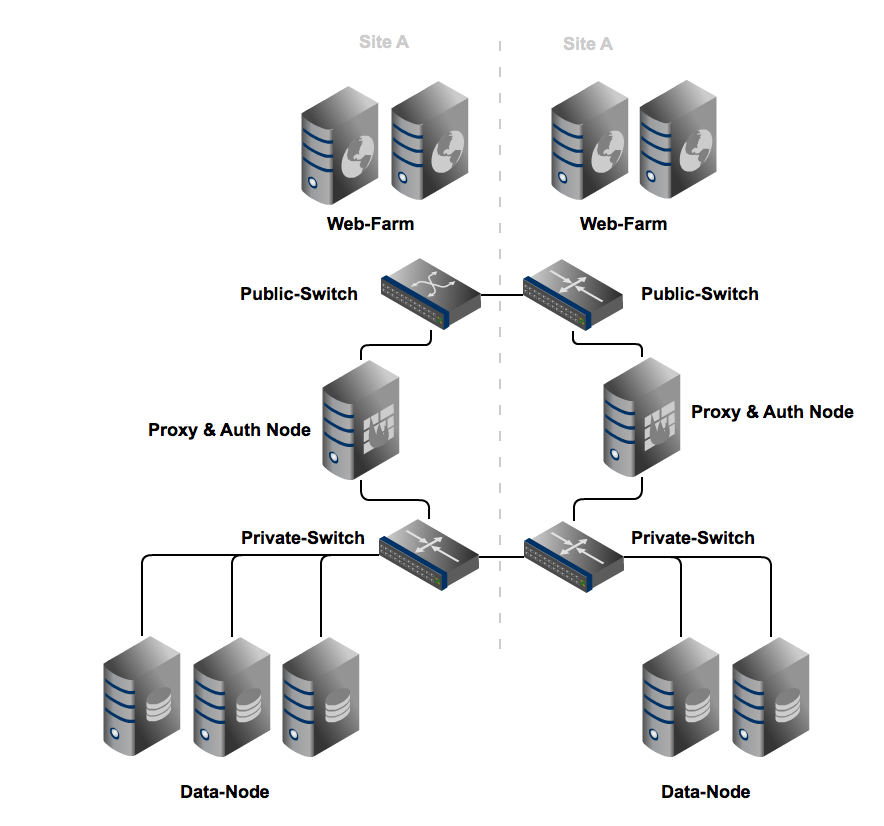
\includegraphics[width=\linewidth, keepaspectratio = true]{media/OpenStack.png}
\mycaption{figure}{\label{abb:OpenStack-Infrastruktur} OpenStack Infrastrutkur}
\end{center}


\subsubsection*{Verfügbarkeit}
OpenStack Object Storage wurde so konzipiert, dass ein Ausfall einer Hardwarekomponente den Weiterbetrieb aufrecht erhalten kann, ohne dabei einen Datenverlust oder die Verfügbarkeit des Systems zu gefährden. Die Daten bzw. Objekte werden redundant auf mehreren Zonen gespeichert. Zonen sind Gruppierungen von Servern. Die Anzahl redundanten Replikate für ein Objekt kann konfiguriert werden. Gewöhnlich werden drei Kopien verwaltet.

Für die Architektur wird von Joe Arnolds CEO bei SwiftStack bei dreifacher Redundanz die Implementierung von 5 Zonen empfohlen. OpenStack Object Storage, speichert die redundanten Objekte jeweils in einer separaten Zonen. Eine Zone kann bei kleinen Implementationen auch nur aus Gruppen von Festplatten bestehen, also innerhalb eines einzigen Servers existieren. Es wird aber empfohlen, eine Zone auf Hierarchie von Server-Gruppen zu implementieren. Das bedeutet, jede redundante Kopie ist auf einem eigenen Server gespeichert. \cite{Arnold} 

Zusätzlich zu den Speicherservern benötigt es noch zwei oder mehrere Proxy Server, um die hohe Verfügbarkeit zu gewährleisten. Die Proxy Server werden bei Rackspace mit 10 Gb Ethernet an den Netzwerk-Switch angeschlossen. \cite{OpenStack2011}

Möchte man den Speicher standortübergreifend betreiben, ist es erforderlich, dass pro Standort nicht mehr als $(Redundanz -1)$ Zonen betrieben werden, da ansonsten die Gefahr besteht, dass alle Replikate am gleichen Standort gespeichert werden. Das möchte niemand.

\subsubsection*{Speicherkapazität}
Der OpenStack Object Storage Cluster lässt sich im laufenden Betrieb ohne Unterbruch vergrössern. In der Regeln können auch Software Updates und Patches ohne Unterbruch des Clusters eingespielt werden, wenn darauf geachtet wird, nie mehr als eine Zone gleichzeitig zu aktualisieren.

Grundsätzlich ist die Anzahl an speicherbaren Objekten nicht begrenzt. Der Container Server von OpenStack Object Storage, dessen primäre Aufgabe es ist, die Auflistung der gespeicherten Objekten in einen Container zu verwalten, speichert die Informationen, welche Objekte sich im Container befinden. Pro Container in ein SQLite Datenbank angelegt. Die Performance der Datenbank, welche mit der Anzahl Einträge abnimmt, kann sich zum limitierenden Faktor entwickeln. Wie viele Objekte in einem Container gespeichert werden können. Der Performance Einbruch kann, je nach Leistung der Hardware und die generelle Last auf dem Cluster, bei ca. einer Million Objekten pro Container eintreten. Es können pro Account mehrere Container erstellt werden, wodurch die Limitierung entschärft wäre. Zu beachten ist hier, dass pro Account ebenfalls eine SQLite Datenbank mit allen Containern geführt wird und auch hier dieselben Einschränkungen zum tragen kommen. \cite{OpenStack2012}\cite{A2011}

\subsubsection*{Datenzugriff}
Der Zugriff auf die gespeicherten Objekten erfolgt ähnlich wie bei Amazon S3 über ein API. Das API verwendet für den Zugriff den standard HTTP Request. Verschiedene Speicherlösungs-Hersteller haben angekündigt, das Swift API ebenfalls für den Zugriff auf ihren Speicher unterstützen zu wollen. Glusterfs mit seiner verteilten Speicherlösung, bietet in der Entwicklerversion bereits die Unterstützung für Swift an. Applikationen, welche, das Swift API unterstützen, können ihre Speicherlösung künftig einfacher austauschen, ohne dabei die Applikation anpassen zu müssen. Neben dem Zugriff mit dem Swift API, bietet OpenStack eine Amazon S3 kompatibles API an. Der Zugriff über POSIX IO auf den Speicher ist nicht möglich.

Der Zugriff auf den Speicher erfolgt über einen Proxy, welcher den Speicherort des Objektes prüft und die Anfrage weiterleitet. Pro OpenStack Object Storage Cluster können mehrere Proxys eingesetzt werden. Mit Hilfe eines Load Balancers (Last Verteiler) können die Anfragen über die vorhandenen Proxys verteilt werden.

Die maximale Uploadgrösse beträgt 5 GB, die Downloadgrösse ist jedoch unbeschränkt. Wenn ein Objekt grösser als 5 GB hochgeladen wird, wird das Objekt in Teilen hochgeladen und gespeichert. Die Abfrage auf das Objekt erfolgt wie bei einem ganzen Objekt. Es müssen also keine Teile durch das API adressiert werden. \cite{OpenStack2012a}


\subsubsection*{Datenschutz}
OpenStack Object Storage stellt die Datenintegrität beim Speichern von Objekten und beim Auslesen der Daten sicher. Somit ist gewährleistet, dass die Daten im original gespeichert werden und bei der Speicherung kein Datenverlust entsteht. Die Selbstheilung von korrupten Objekten stellt OpenStack Objekt Storage mit dem Auditors Dien6st sicher. Der Auditors Dienst läuft auf jedem Server und prüft dort die Integrität von Objekten. Wenn ein korruptes Objekt erkannt wird, wird die Datei sofort unter Quarantäne gestellt und durch ein korrektes Reblikations-Objekt ersetzt.
Um die Last die durch den Auditors möglichst gering zu halten, kann die Anzahl Objekte oder die Anzahl Bits, die pro Sekunde geprüft werden, konfiguriert werden. \cite{OpenStack2012}

OpenStack Objekt Storage bietet neben der Redundanz der Objekte keine Möglichkeit, die Daten zu sichern. Dadurch ist keine Versionierung der Objekte möglich. Zwar lassen sich die Cluster Nodes mit einer konventionellen Sicherungssoftware direkt sichern. Dadurch lässt sich nur der gesamte Cluster wiederherstellen und nicht einzelne Objekte. Zudem wäre die Speicherkapazität pro Sicherung so gross wie es für die redundante Speicherung der Objekte Speicherkapazität benötigt würde. \cite{AndyBrezinsky2011}


Die Sicherheit der Daten wird mit sogenannten Accounts sichergestellt. Das heisst, dass ein Account nur auf seine gespeicherten Objekten zugreifen kann. Die Daten werden auf dem OpenStack Cluster unverschlüsselt in binärer Form gespeichert. Durch die Verteilung der Daten müsste jedoch ein Angreifer Zugriff auf alle Cluster Node erlangen, um an alle Daten eines Account zu gelangen.

\subsubsection*{Technologie}
OpenStack Objekt Storage wurde von der Firma RackSpace unter dem Code Name Swift entwickelt. Zusammen mit National Aeronautics and Space Administration (NASA) hat RackSpace die Softwareprojekt-Gemeinschaft OpenStack gegründet und Swift zusammen mit der Cloud-Lösung Nova für die Verwaltung von virtuellen Maschinen und Glace für die Verwaltung von Images als quelloffene Software veröffentlicht. Die OpenStack Gemeinschaft ist in Vergleich zu anderen quelloffenen Gemeinschaften noch eine relative jung Gemeinschaft. Es gelang ihr dennoch neben den beiden Gründerunternehmen weiter bedeutende Unternehmen aus der Informatikbranche, wie Hewlett Packard, Dell, Citrix, Intel, AMD, NetApp und weitere zu gewinnen. Eine vollständige Liste aller unterstützenden Unternehmen ist unter \url{http://openstack.org/community/companies/} zu finden. Die Aktivität auf der Projektseite von OpenStack Object Storage lässt erkennen, dass die Entwicklung aktiv vorangetrieben wird und viele Beiträge zu neuen Funktionen oder Verbesserungen von Anwendern und Entwickler beigetragen werden. \cite{Ohloh2012}

Die Internet-Recherche für auf OpenStack spezialisierte Schweizer Firmen ergaben keine Ergebnisse. 
Gemäss Internet-Recherchen gibt es noch keine spezialisierten Firmen für OpenStack Lösungen. Einige wenige Experten für OpenStack mit Domizil in der Schweiz konnten über die Profile bei LinkedIn, einem Social Network für Firmen, gefunden werden. 

Für die Verwaltung des Speichers bietet OpenStack ein Kommandozeilen-Tools an. Ein Web-GUI für Objekt Storage von OpenStack gibt es nicht. Die Firma SwiftStack bietet hierfür eine kostenpflichtige Lösung an. Die Überwachung des Speichers, zum Beispiel für die Verfügbarkeit einzelner Cluster Nodes, muss mit zusätzlichen Fremdlösungen erfolgen. 

\subsubsection*{Kosten}
Grundsätzlich unterscheiden sich die Kosten für die beiden Szenario nur in der Anzahl Server, den verwendeten Server Typen, der Anzahl Festplatten und dem benötigten Rackplatz. Die restlichen Faktoren sind für beide Szenarien gleich und werden in diesem Abschnitt behandelt.

Um die Rechenzentrumskosten möglichst tief zu halten, welche pro Rack verrechnet werden, soll möglichst viel Speicherkapazität in einer Rackeinheit gepackt werden. Dies bedeutet, dass die richtigen Server für die Anzahl der zur Verfügung gestellten Speicherkapazität verwendet werden sollen.

Um die Preise für die Festplatten möglichst tief zu halten werden diese separate beschaffen. Als Festplatte soll eine SATA-3 3.5 Zoll 3 Terabyte Festplatte eingesetzt werden. Dies entspricht 2.728 Tebibyte. Die Kosten für Festplatten sind stark marktabhängig, Für die Arbeit wird einfachheitshalber mit ca. 300 CHF pro Festplatte budgetiert.

Für beide Szenarien werden die gleichen Proxy-Server verwendet. Als Proxy Server wurden die Transtec Server-Systeme "'Lynx CALLEO Application Server 2260S'" ausgewählt. Die Proxy Server stammen vom selben Hersteller wie die in den Szenarien aufgeführten Datenserver. Dies hat den Vorteil, dass nur ein Ansprechpartner für die Server-Farm benötigt wird. Es ist kein Muss-Kriterium und kann bei Bedarf durch ein besseres Angebot eines anderen Herstellers ersetzt werden. Die Proxy sind mit einem Intel Xeon Prozessor E5-2665 mit 64 Gigabyte Hauptspeicher ausgerüstet. Die Server haben eine Rack-Höheneinheit von je 2 Einheiten. Wie bei den Datenserver wurde ein 365 mal 24 Stunden vor Ort Service ausgewählt. Der Preis pro Server beträgt 9'954 CHF.

Neben der Server Infrastruktur sind noch zwei Netzwerk-Switches notwendig. Der Dell PowerConnect 8024 bietet 24 Port mit 10GbE. Die Switches haben eine Rack-Höheneinheit von je 1 Einheiten und benötigen gemäss Hersteller maximal 237,77 Watt. Dell gewährt einen 3 Jahres Support für den Switch. Der Preis pro Switch beträgt 14'732 CHF.

Als Rechenzentrumsbetreiber wurde Nine Internet Solution ausgewählt. Nine betreibt ihr Rechenzentrum in Zürich und ist auf das Hosting spezialisiert. Mit seinem Rechenzentrumsstandort in der Stadt Zürich befindet sich Nine geographisch in der Nähe des Auftraggebers. Die Anfahrtszeit und der Anfahrtsweg kann so für den Auftraggeber kurz gehalten werden. Die verschiedenen Rack-Produkte, welche Nine anbietet, unterscheiden sich von der Anzahl Rack-Höheneinheiten und deren Watt-Leistung. In den Produkten ist zusätzlich die Anbindung ans Internet mit 100 Mbps enthalten. Bei zusätzlichem Wattbedarf bietet Nine die Möglichkeit, die zusätzliche Watts in 500er Pakete zu 165 CHF pro Monat an.

Für den den Betrieb der Speicherinfrastruktur wird mit einer Mannstelle gerechnet. Organisatorisch kann diese auch auf mehrere teilprozentuale Stellen aufgeteilt werden, damit auch der Betrieb während Ferienabwesenheiten sichergestellt ist. Pro Monat wird mit Personalkosten von 15'000 CHF gerechnet.


\paragraph*{Kosten Szenario-1}

Für die dreifache Redundanz sind für die aus der Soll-Analyse bestimmten 306 Tebibyte gemäss \refeqlb{eqn:SpeicherkapazitätS1} 918 Tebibyte an Speicherkapazität notwendig.

\begin{equation}
\mbox{Speicherkapazität}_{Redundanz} = 306 \mathrm{\ TiB} * 3 \mbox{\ Redundanz} = 918 \mathrm{\ TiB}
\label{eqn:SpeicherkapazitätS1}
\end{equation}


Als Server System wurde der Transtec Lynx CALLEO Application Server 1260 gewählt. Der Server basiert auf Server-Hardware des Herstellers SuperMicro. Der Server benötigt 1 Rack-Höcheneinheiten und bietet Platz für den Einbau von 4 3.5 Zoll Festplatten, welche auch während des Betriebs ausgetauscht werden können. Als Prozessoreinheit kommen ein Intel Xeon Prozessor E5-2620 zum Einsatz. Ferner verfügt der Server über 32 Gigabyte Hauptspeicher. Der Server wurde mit einem 3 Jahres, 24 Stunden, 365 Tage Vor-Ort Service gerechnet. Somit ist sichergestellt, dass im Störungsfall der Unterbruch möglichst gering gehalten werden kann. Der Preis pro Server beträgt ohne Festplatten 1'260 CHF.


Ein Server mit Festplatten ausgerüstet, weist gemäss der \refeqlb{eqn:SpeicherkapazitätServerS1} eine Speicherkapazität von 10,912 Tebibyte aus. Damit sind in anbetracht der notwendigen Speicherkapazität von 48,3 Tebibyte und der 5 Zonen insgesamt 5 Server notwendig (siehe \refeqlb{eqn:AnzahlServerS1}). Für die Speicherkapazität von 48,3 Tebibyte bei gleich ausgerüsteten Servern sind insgesamt nur 20 Festplatten notwendig.

\begin{equation}
\mbox{Speicherkapazität}_{Server} = 2,728 \mathrm{\ TiB} * 4 \mbox{\ Einschub} = 10,912 \mathrm{\ TiB}
\label{eqn:SpeicherkapazitätServerS1}
\end{equation}

\begin{equation}
\mbox{Anzahl Server} = \frac{48,3 \mathrm{\ TiB}}{10,912 \mathrm{\ TiB}} \approx 5 \mbox{\ (Auf 5 Zonen gerundet)}
\label{eqn:AnzahlServerS1}
\end{equation}

\begin{equation}
\mbox{Anzahl Festplatten} = \frac{48,3 \mathrm{\ TiB}}{2,728 \mathrm{\ TiB}} \approx 20 \mbox{\ (Auf 5 Server gerundet)}
\label{eqn:AnzahlFestplattenS1}
\end{equation}

Gemäss \refeqlb{eqn:AnzahlRackS1} wird ein viertel-Rack für den Einbau aller Komponenten benötigt. Der Rackplatz entspricht dem Quarter Rack Angebot von Nine, welches 11 Rack-Höheneinheiten platz bietet. Der Preis pro Rack beträgt 450 CHF pro Monat, plus 650 CHF für die einmalige Einrichtung des Racks durch Nine.
Für die Berechnung der Gesamt Watt-Leistung fehlen die Angaben des Herstellers. Aus diesem Grund wird angenommen, dass der Daten-Server ca. 300 Watt und der Proxy-Server ca. 500 Watt bezieht. Mit diesen Annahmen benötigt es gemäss \refeqlb{eqn:AnzahlWattPaketeS1}, die 500 Watt, welche im Rackpreis enthalten sind, zusätzliche 5 Pakete a je 500 Watt pro Monat.

\begin{equation}
\mbox{Anzahl Racks} = \frac{5 * 1 \mathrm{\ U} + 2 * 2 \mathrm{\ U} + 2 * 2 \mathrm{\ U}}{11\mathrm{\ U}} \approx 1 \mbox{\ (Auf viertel Rack gerundet)}
\label{eqn:AnzahlRackS1}
\end{equation}

\begin{equation}
\mbox{Anzahl 500 \mathrm{W} Pakete} = \frac{5 * 300 \mathrm{\ W} + 2 * 500 \mathrm{\ W} +2 * 237,77 \mathrm{\ W} - 2000 \mathrm{\ W} }{500\mathrm{\ W}} \approx 5
\label{eqn:AnzahlWattPaketeS1}
\end{equation}

Wie aus der \reftab{tab:KostenOpenStackS1} ersichtlich ist, betragen die Gesamtkosten 653'646.50 CHF.


\begin{table}[htbp]
\caption{Kosten OpenStack Szenario-1}
\begin{small}
\begin{tabular}{|l|r|r|r|}
\hline
\textbf{Beschreibung} & \multicolumn{1}{l|}{\textbf{Kosten pro Stk/M.}} & \multicolumn{1}{l|}{\textbf{Anzahl}} & \multicolumn{1}{l|}{\textbf{Total}} \\ \hline
 \multicolumn{ 4}{c}{} \\ \hline
\multicolumn{ 4}{|c|}{\textbf{Investitionskosten}} \\ \hline
Dell PowerConnect 8024 & CHF 14'732.00 & 2 & CHF 29'464.00 \\ \hline
Lynx CALLEO App. Server 1260 & CHF 5'451.50 & 2 & CHF 10'903.00 \\ \hline
Lynx CALLEO App. Server 1260 & CHF 2'831.30 & 5 & CHF 14'156.50 \\ \hline
Festplatte 3,5 3 TB & CHF 300.00 & 20 & CHF 6'000.00 \\ \hline
Rack Einrichtung & CHF 650.00 & 1 & CHF 650.00 \\ \hline \hline
 \multicolumn{ 3}{r|}{\textbf{Total:}} & \textbf{CHF 61'173.50} \\ 
 \cline{4-4}
\multicolumn{ 4}{c}{} \\ \hline
\multicolumn{ 4}{|c|}{\textbf{Fortlaufende Kosten}} \\ \hline
Dell Service & CHF 0.00 & 2 & CHF 0.00 \\ \hline
Transtec Service (Server 1260) & CHF 26.08 & 2 & CHF 52.17 \\ \hline
Transtec Service (Server 1260) & CHF 26.08 & 5 & CHF 130.42 \\ \hline
Rackkosten 11 U (500 W) & CHF 450.00 & 1 & CHF 450.00 \\ \hline
Strom 500 W & CHF 165.00 & 5 & CHF 825.00 \\ \hline
Personal & CHF 15'000.00 & 1 & CHF 15'000.00 \\ \hline \hline
 \multicolumn{ 3}{r|}{\textbf{Total pro Monat:}} & CHF 16'457.58 \\
\cline{4-4}
 \multicolumn{ 3}{r|}{\textbf{Total 36 Monate:}} & \textbf{CHF 592'473.00} \\ \cline{4-4}
 \multicolumn{ 4}{c}{} \\ \cline{4-4}
 \multicolumn{ 3}{r|}{\textbf{Total Gesamt:}} & \textbf{CHF 653'646.50} \\ \cline{4-4}
\end{tabular}
\end{small}
\label{tab:KostenOpenStackS1}
\end{table}



\paragraph*{Kosten Szenario-2}

Für die dreifache Redundanz sind für die aus der Soll-Analyse bestimmten 306 Tebibyte gemäss \refeqlb{eqn:SpeicherkapazitätS2} 918 Tebibyte an Speicherkapazität notwendig.

\begin{equation}
\mbox{Speicherkapazität}_{Redundanz} = 306 \mathrm{\ TiB} * 3 \mbox{\ Redundanz} = 918 \mathrm{\ TiB}
\label{eqn:SpeicherkapazitätS2}
\end{equation}


Als Server-System wurde der Transtec Lynx CALLEO Application Server 4260 gewählt. Der Server basiert auf Server-Hardware des Herstellers SuperMicro, welche gemäss eigenen Recherchen auch bei anderen OpenStack Lösungen verwendet wird. Der Server benötigt 4 Rack-Höcheneinheiten Platz und bietet Platz für den Einbau von 36 3.5 Zoll Festplatten, welche auch während des Betriebs ausgetauscht werden können. Als Prozessoreinheit kommen zwei Intel Xeon Prozessor E5-2620 zum Einsatz. Ferner verfügt der Server über 64 Gigabyte Hauptspeicher. Der Server wurde mit einem 3 Jahres, 24 Stunden, 365 Tage Vor-Ort Service gerechnet. Somit ist sichergestellt, das im Störungsfall der Unterbruch möglichst gering gehalten werden kann. Der Preis pro Server beträgt ohne Festplatten 8'672 CHF.


Ein Server ausgerüstet mit Festplatten weist gemäss der \refeqlb{eqn:SpeicherkapazitätServerS2} eine Speicherkapazität von 98.208 Tebibyte aus. Damit sind in anbetracht der notwendigen Speicherkapazität von 918 Tebibyte und der 5 Zonen insgesamt 10 Server notwendig (siehe \refeqlb{eqn:AnzahlServerS2}). Für die Speicherkapazität von 918 Tebibyte bei gleich ausgerüsteten Servern sind insgesamt nur 340 Festplatten notwendig. Das heisst, pro Server sind 34 Einschübe mit Festplatten belegt. Sie könnten bei Bedarf noch weiter aufgerüstet werden.

\begin{equation}
\mbox{Speicherkapazität}_{Server} = 2,728 \mathrm{\ TiB} * 36 \mbox{\ Einschub} = 98.208 \mathrm{\ TiB}
\label{eqn:SpeicherkapazitätServerS2}
\end{equation}

\begin{equation}
\mbox{Anzahl Server} = \frac{918 \mathrm{\ TiB}}{98.208 \mathrm{\ TiB}} \approx 10 \mbox{\ (Auf 5 Zonen gerundet)}
\label{eqn:AnzahlServerS2}
\end{equation}

\begin{equation}
\mbox{Anzahl Festplatten} = \frac{918 \mathrm{\ TiB}}{2,728 \mathrm{\ TiB}} \approx 340 \mbox{\ (Auf 10 Server gerundet)}
\label{eqn:AnzahlFestplattenS2}
\end{equation}

Gemäss \refeqlb{eqn:AnzahlRackS2} wird ein ganzes Rack für den Einbau aller Komponenten benötigt. Der Rackplatz entspricht den Full Rack Angebot von Nine, welches 47 Rack-Höheneinheiten platz bietet. Der Preis pro halbes Rack beträgt 750 CHF pro Monat, plus 850 CHF für die einmalige Einrichtung des Racks durch Nine.
Für die Berechnung der Gesamt Watt-Leistung fehlen die Angaben des Herstellers. Aus diesem Grund wird angenommen, dass der Daten-Server ca. 700 Watt und der Proxy-Server ca. 500 Watt bezieht. Mit diesen Annahmen benötigt es gemäss \refeqlb{eqn:AnzahlWattPaketeS2}, den 2000 Watt, welche im Rackpreis enthalten sind, zusätliche 13 Pakete zu je 500 Watt pro Monat.

\begin{equation}
\mbox{Anzahl Racks} = \frac{10 * 4 \mathrm{\ U} + 2 * 2 \mathrm{\ U} + 2 * 2 \mathrm{\ U}}{47\mathrm{\ U}} \approx 1 \mbox{\ (Auf ganze Rack gerundet)}
\label{eqn:AnzahlRackS2}
\end{equation}

\begin{equation}
\mbox{Anzahl 500 \mathrm{W} Pakete} = \frac{10 * 700 \mathrm{\ W} + 2 * 500 \mathrm{\ W} +2 * 237,77 \mathrm{\ W} - 2000 \mathrm{\ W} }{500\mathrm{\ W}} \approx 13
\label{eqn:AnzahlWattPaketeS2}
\end{equation}

Wie aus der \reftab{tab:KostenOpenStackS2} ersichtlich ist, betragen die Gesamtkosten 916'965.00 CHF.

\begin{table}[htbp]
\caption{Kosten OpenStack Szenario-2}
\begin{small}
\begin{tabular}{|l|r|r|r|}
\hline
\textbf{Beschreibung} & \multicolumn{1}{l|}{\textbf{Kosten pro Stk/M.}} & \multicolumn{1}{l|}{\textbf{Anzahl}} & \multicolumn{1}{l|}{\textbf{Total}} \\ \hline
 \multicolumn{ 4}{c}{} \\ \hline
\multicolumn{ 4}{|c|}{\textbf{Investitionskosten}} \\ \hline
Dell PowerConnect 8024 & CHF 14'732.00 & 2 & CHF 29'464.00 \\ \hline
Lynx CALLEO App. Server 1260 & CHF 5'451.50 & 2 & CHF 10'903.00 \\ \hline
Lynx CALLEO App. Server 4260H & CHF 6'111.00 & 10 & CHF 61'110.00 \\ \hline
Festplatte 3,5 3 TB & CHF 300.00 & 340 & CHF 102'000.00 \\ \hline
Rack Einrichtung & CHF 850.00 & 2 & CHF 1700.00 \\ \hline \hline
Mulit-Site Einrichtung & CHF 1500.00 & 1 & CHF 1500.00 \\ \hline \hline
 \multicolumn{ 3}{r|}{\textbf{Total:}} & \textbf{CHF 206'677.00} \\ \cline{4-4}
\multicolumn{ 4}{c}{} \\ \hline
\multicolumn{ 4}{|c|}{\textbf{Fortlaufende Kosten}} \\ \hline
Dell Service & CHF 0.00 & 2 & CHF 0.00 \\ \hline
Transtec Service (Server 1260) & CHF 26.08 & 2 & CHF 52.17 \\ \hline
Transtec Service (Server 4260H) & CHF 53.31 & 10 & CHF 533.06 \\ \hline
Rackkosten 22 U (1000 W) & CHF 750.00 & 2 & CHF 1'500.00 \\ \hline
Strom 500 W & CHF 165.00 & 13 & CHF 2'145.00 \\ \hline
Mulit-Site 1 GBit/s & CHF 500.00 & 1 & CHF 500.00 \\ \hline
Personal & CHF 15'000.00 & 1 & CHF 15'000.00 \\ \hline \hline
 \multicolumn{ 3}{r|}{\textbf{Total pro Monat:}} & CHF 19'730.22 \\ \cline{4-4}
 \multicolumn{ 3}{r|}{\textbf{Total 36 Monate:}} & \textbf{CHF 710'288.00} \\ \cline{4-4}
 \multicolumn{ 4}{c}{} \\ \cline{4-4}
 \multicolumn{ 3}{r|}{\textbf{Total Gesamt:}} & \textbf{CHF 916'965.00} \\ \cline{4-4}
\end{tabular}
\end{small}
\label{tab:KostenOpenStackS2}
\end{table}


\subsection{\ref{Al-5}: Amazon S3}
Amazon zählt zu den grössten, wenn nicht der grösste Online Speicheranbieter weltweit. Genaue Angaben über die Anzahl Kunden und Speicherkapazität veröffentlich Amazon nicht. Seit 2006 bietet Amazon Ihren Kunden unter dem Produktname S3, einen Online Speicher an. Die genaueren technischen Eigenschaften und Architektur des Online Speicher ist bis anhin von Amazon nicht veröffentlicht worden. Nach eigenen Angaben von Amazon basiert die Dienstleistung auf gewöhnlicher Computer Hardware.

Im \refabb{abb:AmazonS3-Infrastruktur} ist die Netzwerk und System-Architektur dargestellt. Es zeigt wie die Applikations-Server Farm Bildobjekte über das Internet auf dem Amazon S3 Speicher ablegt und darauf zugreift. Zudem zeigt die Abbildung wie eine Client-Anfrage auf ein Bildobjekt an die Applikations-Server Farm, den direkten URL Pfad zum Bildobjekt auf den Amazon S3 Speicher verweist. Somit kann die Auslieferung der Bilddaten direkt über Amazon S3 erfolgen, was die Bandbreite der Applikations-Server Farm entlastet. 

\begin{center}
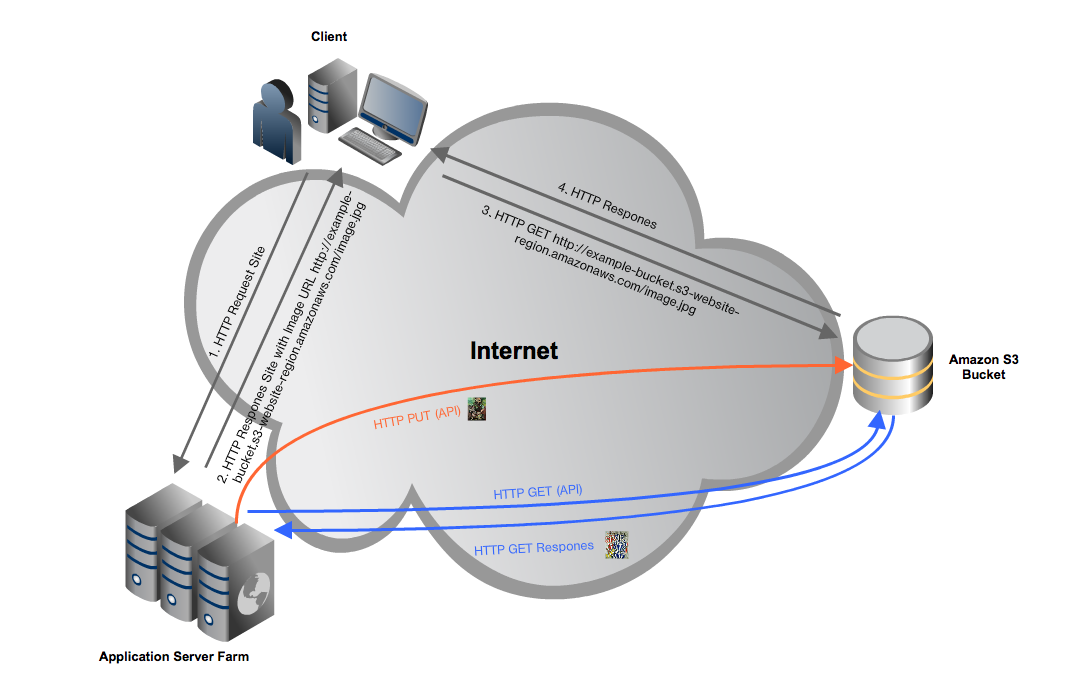
\includegraphics[width=\linewidth, keepaspectratio = true]{media/Amazon_S3.png}
\mycaption{figure}{\label{abb:AmazonS3-Infrastruktur} Amazon S3 Netz und System Architektur}
\end{center}




Bei Online Speicher wie Amazon S3, kann der Kunde gleich nach Anmeldung an den Dienst, die Speicherressourcen verwenden. Es fallen also keine Installationkosten für die Speicherinfrastruktur an. 

\subsubsection*{Verfügbarkeit}
Amazon S3 speichert die Daten auf mehreren Geräten in verschiedenen Rechenzentren in derselben Region ab. Beim Speichern werden die Daten synchron in verschiedene Rechenzentren abgelegt bevor die Speicherung als erfolgreich gemeldet wird. Damit ist sichergestellt, dass die Daten von Beginn weg einwandfrei redundant gespeichert sind. Mit diesen Massnahmen gewährleistet Amazon gemäss Dienstgütevereinbarung eine Zuverlässigkeit von 99.999999999\%. Bei Bedarf kann die Zuverlässigkeit für Daten, welche wenig Schutz benötigen, wie zum Beispiel Thumbnails von Bilder, mit einer geringeren Zuverlässigkeit von 99.99\% zu einem günstigeren Preis gespeichert werden. \cite{Amazon2007}

Durch die redundante Speicherung der Daten auf mehrere Geräte gewährleistet Amazone gemäss Dienstgütevereinbarung von 99.99\% pro Monat.

\subsubsection*{Datenzugriff}
Der Zugriff auf die Daten findet über eine API oder über die Verwaltungskonsole von Amazon statt. Für den Zugriff mit einem API bietet Amazon ein \gls{REST} und eine \gls{SOAP} Schnittstelle an. Der \gls{REST} Zugriff findet über HTTP statt. Dabei werden standard HTTP requests verwendet. Für den Zugriff kann auch ein gewöhnlicher Web-Browser verwendet werden solange die Objekte öffentlich sind.

Einen offiziellen POSIX IO Zugriff von Amazon steht nicht zur Verfügung. Es existiert allerdings ein quelloffenes Projekt Namens s3fs\footnote{\url{https://code.google.com/p/s3fs/}}, welches es ermöglicht, einen Amazon S3 Speicher unter Linux zu mounten. \cite{S3fs}

Da die Infrastruktur von Amazon S3 nicht bekannt ist, können keine detaillierten Angaben über die Skalierung der Datenzugriffe gemacht werden. Es kann von einem hochskalierbaren System ausgegangen werden, da Amazon die Zugriffe von tausenden von Kunden gleichzeitig handhaben muss.

Amazon S3 unterstützt das Lesen und Schreiben von mehreren Systemen. Beim Lesen einen Objektes, welches aus mehreren Systemen zugegriffen und beschrieben wird, stellt Amazon S3 die Lesekonsistenz sicher. \cite{Amazon2012a}

Für das Einlesen von grossen Datenmengen bietet Amazon einen kostenpflichtigen Import/Export Dienstleistung an. Bei dieser Dienstleistung sendet der Kunde die Daten gespeichert auf einem tragbaren Speichermedium an Amazon, welches die Daten direkt in ihre Cloud ohne Umwege über das Internet einliesst.

Die API von Amazon ist gut dokumentiert, weshalb für einen erfahrenen Entwickler die Anbindung der Web-Applikation an Amazon S3 umsetzbar sein sollte.

\subsubsection*{Speicherkapazität}
Für die Skalierung der Speicherkapazität kümmert sich Amazon.

Im Amazon S3 können eine unbegrenzte Anzahl von Objekten gespeichert werden, welche eine Speichergrösse von 1 Byte bis zu 5 Terrabyte haben können. In einem PUT können maximal 5 Gigabyte hochgeladen werden. Für das Hochladen von grösseren Objekten muss die Multipart Funktion verwendet werden, welche das Objekte in mehrere Teilen gliedert und hochladet. \cite{Amazon2012b}

\subsubsection*{Datenschutz}
Die Daten können bei Amazon in mehren Regionen gespeichert werden. Zu den verfügbaren Regionen gehören, US Standard, US West (Oregon), US West (Northern California), EU (Ireland), Asia Pacific (Singapore), Asia Pacific (Tokyo), South America (Sao Paulo). Gemäss Amazon verlassen die gespeicherten Daten eine Region nicht, ausser für die Erfüllung von Gesetzen oder auf Anforderung einer Regierung. Als US amerikanisches Unternehmen steht Amazon wegen dem Patriot Act unter der Pflicht, den US-Behörden auf Anforderung Zugang zu den Daten zu gewährleisten, auch wenn diese Informationen ausserhalb der USA gespeichert sind. Gemäss EU Recht dürfen ohne Einverständnis der Behörden keine gespeicherten Informationen an Dritten zugänglich gemacht werden, auch nicht solche Daten die ausserhalb der EU gespeichert sind. Bei Microsoft, ebenfalls ein grosser Cloud-Anbieter bestätigt diese Regel, dass die Daten nicht vor dem Zugriff der USA geschützt sind. \cite{Amazon2012}\cite{Ostler}

Die Integrität der Daten wird mit einer Prüfsumme sichergestellt. Die gespeicherten Daten werden von Amazon regelmässig auf ihre Integrität geprüft und bei Bedarf von einer integren Kopie der Daten ersetzt. 

Die Daten können verschlüsselt per SSL zugegriffen bzw. gespeichert werden. Somit ist gewährleistet, dass Dritte die Daten beim Transport nicht lesen können. Seit 2011 bietet Amazon kostenlos ebenfalls die Verschlüsselung mit AES-256 von Objekten im Speicher an. Dabei wird jedes Objekt mit einem eigenen Schlüssel ver- und entschlüsselt. Die erzeugten Schlüssel werden mit einem Master-Schlüssel ebenfalls verschlüsselt und auf den Amazon-Servern gespeichert. Das Schlüsselmanagment bleibt jedoch bei Amazon, weshalb man abhängig von den Massnahmen zum Schutz des Schlusselmanagment ist die Amazon alleine trifft. Wird diese kompromitiert oder fällt sie aus, ist der Zugriff auf die verschlüsselten Daten nicht mehr möglich. \cite{RobertLippert2011}

Die Berechtigung auf gespeicherte Objekte oder Ordner können mit einem Rechte-Management verwaltet werden. Objekte können öffentlich zugänglich gemacht werden oder nur an bestimmte authentifizierte Benutzer zur Verfügung gestellt werden. Zudem lassen sich Zugriffe auf Objekte protokollieren. \cite{Amazon2012b}

Für die Berechtigung und Verwaltung stellt Amazon ein Web-GUI zur Verfügung. Bis auf das Eröffnen eines Speichers und die Initialberechtigung sollten voraussichtlich nicht weitere Verwaltungsaufgaben anfallen.

Amazon bietet neben der Redundanz der Objekte kein weiteres Sicherungsverfahren an. Beim Herunterladen der Daten fallen für den Transfer zusätzliche Kosten an.

\subsubsection*{Technologie}
Der Online Speicher von Amazon S3 gilt als ausgereiftes und etabliertes Produkt im Markt. Es kann davon ausgegangen werden, dass die Dienstleistung über die nächsten vier Jahre hinaus bestehen wird und für den Kunden keine Migration notwendig ist. Amazon S3 wird ebenfalls von SmugMug, ein Photodienstleister, verwendet oder andere bekannte Web-Applikationen wie Dropbox verwendet. \cite{SmugMug}\cite{Dropbox2011}

Der Online-Speicher-Markt ist im Verhältnis zu anderen Speichermärkten noch relativ jung. Analysten wie Jeff Boles gehen davon aus, dass der Online-Speicher-Markt in den nächsten Jahren stark wachsen wird. Wie in der Marktstudie beschrieben, konnte Amazon seit dem Start des Amazon S3 Produktes die Anzahl gespeicherte Objekte jeweils pro Jahr mehr als verdoppeln (sie dazu \refabb{abb:AnzahlObjekteAmazonS3}). Die Konkurrenz wie Google, Microsoft oder Rackspace machen Amazon den Markt streitig. Der Kunden darf hoffen, dass die Anbieter ihre Preise noch spitzer kalkulieren müssen, um konkurrenzfähig zu bleiben. Amazon hat die Preise für S3 Speicher erst kürzlich angepasst. \cite{Boles2011}\cite{Barr2012a}


\subsubsection*{Kosten}
Durch den Bezug der Speicherressourcen als Dienstleistung fallen für den Kunden keine Investitionskosten für die Speicherinfrastruktur an.
Dafür muss in den meisten Fällen die Applikation für den Zugriff mittels Amazon S3 API programmiert werden, wodurch Entwicklungskosten anfallen können.

Beim Amazon S3 wird jeweils nur der effektiv verwendete Speicherplatz pro Monat verrechnet. Im Preis von Amazon ist jeweils die dreifache Redundanz inbegriffen. Der Speicherplatz kostet ab 1 Terabyte bis 49 Terabyte \$ 0.110 per Gigabyte. Ab 49 Terabyte bis 450 Terabyte reduzieren sich die Kosten pro Gigabyte auf \$ 0.095. Anders als beim Betrieb einer eigenen Speicherinfrastruktur muss der Kunden keine zusätzliche Speicherkapazitätsreserven für Unvorhergesehenes einrechnen, da diese erst bei Bedarf von Amazon zur Verfügung gestellt wird. Dies spart substantiell Kosten für den Kunden.

Bei Verwendung von Amazon S3 fallen für den Kunden zudem keine Wartungskosten für den Betrieb der Speicherinfrastruktur an. 

Im Vergleich zum eigenen Betrieb fallen dem Kunden allerdings Kosten für den Transfer und Abfragen der Daten an. So kostet der Transfer der Daten aus dem Amazon S3 Speicher für jedes GB \$ 0.12 bei einem Transfervolumen bis zu 10 TB. Für die Abfrage wird unterschieden zwischen schreibenden und lesenden Abfragen. Der Lesezugriff kostet pro 10'000 Abfragen \$ 0.01 und für jeden Schreibzugriff pro 1'000 Abfragen \$ 0.01. Die tatsächlichen Kosten sind schwierig vorherzusagen und könnten zu Überraschungen führen. Die zu budgetierenden Kosten sind stark von den Anzahl Benutzern und deren Benutzerverhalten abhängig und können saisonalen Schwankungen unterliegen.

\paragraph*{Kosten Szenario-1}
Die Kosten für Szenario-1 betragen gemäss Zusammenstellung der\reftab{tab:KostenAmazonS3S1} total \$ 42'646.32. Das entspricht zum aktuellen Tageskurs gerechnet (13 April 2012) 39'10.52 CHF. 


\subsubsection**{Kosten Szenario-2}
Die Kosten für Szenario-1 betragen gemäss Zusammenstellung der \reftab{tab:KostenAmazonS3S2} total \$ 493'902.84. Das entspricht zum aktuellen Tageskurs gerechnet (13 April 2012) 450'637.17 CHF. 

\begin{table}
\caption{Kosten Amazon S3 Szenario-1}
\begin{center}
\begin{tabular}{|l|r|r|r|}
\hline
\multicolumn{1}{|l|}{\textbf{Bezeichnung}} &\multicolumn{1}{|l|}{\textbf{Monat}} & \multicolumn{1}{l|}
{\textbf{Speicherkapazität}} & \multicolumn{1}{l|}{\textbf{Kosten}} \\ \hline
\multicolumn{4}{c}{} \\ \hline
\multicolumn{ 4}{|c|}{\textit{Investitionskosten}} \\ \hline 
- & & & \\ \hline
\multicolumn{3}{r|}{\textbf{Total:}} & CHF 0.00 \\ \cline{4-4}
\multicolumn{4}{c}{} \\ \hline
\multicolumn{ 4}{|c|}{\textit{Fortlaufende Kosten}} \\ \hline
Amazon S3 & 1 & 2,75 & \$691.82 \\ \hline
Amazon S3 & 2 & 3 & \$719.98 \\ \hline
Amazon S3 & 3 & 3,25 & \$748.14 \\ \hline
Amazon S3 & 4 & 3,5 & \$776.30 \\ \hline
Amazon S3 & 5 & 3,75 & \$804.46 \\ \hline
Amazon S3 & 6 & 4 & \$832.62 \\ \hline
Amazon S3 & 7 & 4,25 & \$860.78 \\ \hline
Amazon S3 & 8 & 4,5 & \$888.94 \\ \hline
Amazon S3 & 9 & 4,75 & \$917.10 \\ \hline
Amazon S3 & 10 & 5 & \$945.26 \\ \hline
Amazon S3 & 11 & 5,25 & \$973.42 \\ \hline
Amazon S3 & 12 & 5,5 & \$1'001.58 \\ \hline
Amazon S3 & 13 & 5,75 & \$1'029.74 \\ \hline
Amazon S3 & 14 & 6 & \$1'057.90 \\ \hline
Amazon S3 & 15 & 6,25 & \$1'086.06 \\ \hline
Amazon S3 & 16 & 6,5 & \$1'114.22 \\ \hline
Amazon S3 & 17 & 6,75 & \$1'142.38 \\ \hline
Amazon S3 & 18 & 7 & \$1'170.54 \\ \hline
Amazon S3 & 19 & 7,25 & \$1'198.70 \\ \hline
Amazon S3 & 20 & 7,5 & \$1'226.86 \\ \hline
Amazon S3 & 21 & 7,75 & \$1'255.02 \\ \hline
Amazon S3 & 22 & 8 & \$1'283.18 \\ \hline
Amazon S3 & 23 & 8,25 & \$1'311.34 \\ \hline
Amazon S3 & 24 & 8,5 & \$1'339.50 \\ \hline
Amazon S3 & 25 & 8,75 & \$1'367.66 \\ \hline
Amazon S3 & 26 & 9 & \$1'395.82 \\ \hline
Amazon S3 & 27 & 9,25 & \$1'423.98 \\ \hline
Amazon S3 & 28 & 9,5 & \$1'452.14 \\ \hline
Amazon S3 & 29 & 9,75 & \$1'480.30 \\ \hline
Amazon S3 & 30 & 10 & \$1'508.46 \\ \hline
Amazon S3 & 31 & 10,25 & \$1'536.62 \\ \hline
Amazon S3 & 32 & 10,5 & \$1'564.78 \\ \hline
Amazon S3 & 33 & 10,75 & \$1'592.94 \\ \hline
Amazon S3 & 34 & 11 & \$1'621.10 \\ \hline
Amazon S3 & 35 & 11,25 & \$1'649.26 \\ \hline
Amazon S3 & 36 & 11,5 & \$1'677.42 \\ \hline
\multicolumn{3}{r|}{\textbf{Total:}} & \textbf{\$ 42'646.32} \\ \cline{4-4}
\multicolumn{4}{c}{} \\ \cline{4-4}
\multicolumn{3}{r|}{\textbf{Total Gesamt:}} & \textbf{ \$ 42'646.32} \\ \cline{4-4}
\end{tabular}
\end{center}
\label{tab:KostenAmazonS3S1}
\end{table}

\begin{table}
\caption{Kosten Amazon S3 Szenario-2}
\begin{center}
\begin{tabular}{|l|r|r|r|}
\hline
\multicolumn{1}{|l|}{\textbf{Bezeichnung}} &\multicolumn{1}{|l|}{\textbf{Monat}} & \multicolumn{1}{l|}
{\textbf{Speicherkapazität}} & \multicolumn{1}{l|}{\textbf{Kosten}} \\ \hline
\multicolumn{4}{c}{} \\ \hline
\multicolumn{ 4}{|c|}{\textit{Investitionskosten}} \\ \hline 
- & & & \\ \hline
\multicolumn{3}{r|}{\textbf{Total:}} & CHF 0.00 \\ \cline{4-4}
\multicolumn{4}{c}{} \\ \hline
\multicolumn{ 4}{|c|}{\textit{Fortlaufende Kosten}} \\ \hline
Amazon S3 & 1 & 8.5 & \$2'937.87 \\ \hline
Amazon S3 & 2 & 14.5 & \$3'613.71 \\ \hline
Amazon S3 & 3 & 20.5 & \$4'289.55 \\ \hline
Amazon S3 & 4 & 26.5 & \$4'965.39 \\ \hline
Amazon S3 & 5 & 32.5 & \$5'641.23 \\ \hline
Amazon S3 & 6 & 38.5 & \$6'317.07 \\ \hline
Amazon S3 & 7 & 44.5 & \$6'992.91 \\ \hline
Amazon S3 & 8 & 50.5 & \$7'661.07 \\ \hline
Amazon S3 & 9 & 56.5 & \$8'244.75 \\ \hline
Amazon S3 & 10 & 62.5 & \$8'828.43 \\ \hline
Amazon S3 & 11 & 68.5 & \$9'412.11 \\ \hline
Amazon S3 & 12 & 74.5 & \$9'995.79 \\ \hline
Amazon S3 & 13 & 80.5 & \$10'579.47 \\ \hline
Amazon S3 & 14 & 86.5 & \$11'163.15 \\ \hline
Amazon S3 & 15 & 92.5 & \$11'746.83 \\ \hline
Amazon S3 & 16 & 98.5 & \$12'330.51 \\ \hline
Amazon S3 & 17 & 104.5 & \$12'914.19 \\ \hline
Amazon S3 & 18 & 110.5 & \$13'497.87 \\ \hline
Amazon S3 & 19 & 116.5 & \$14'081.55 \\ \hline
Amazon S3 & 20 & 122.5 & \$14'665.23 \\ \hline
Amazon S3 & 21 & 128.5 & \$15'248.91 \\ \hline
Amazon S3 & 22 & 134.5 & \$15'832.59 \\ \hline
Amazon S3 & 23 & 140.5 & \$16'416.27 \\ \hline
Amazon S3 & 24 & 146.5 & \$16'999.95 \\ \hline
Amazon S3 & 25 & 152.5 & \$17'583.63 \\ \hline
Amazon S3 & 26 & 158.5 & \$18'167.31 \\ \hline
Amazon S3 & 27 & 164.5 & \$18'750.99 \\ \hline
Amazon S3 & 28 & 170.5 & \$19'334.67 \\ \hline
Amazon S3 & 29 & 176.5 & \$19'918.35 \\ \hline
Amazon S3 & 30 & 182.5 & \$20'502.03 \\ \hline
Amazon S3 & 31 & 188.5 & \$21'085.71 \\ \hline
Amazon S3 & 32 & 194.5 & \$21'669.39 \\ \hline
Amazon S3 & 33 & 200.5 & \$22'253.07 \\ \hline
Amazon S3 & 34 & 206.5 & \$22'836.75 \\ \hline
Amazon S3 & 35 & 212.5 & \$23'420.43 \\ \hline
Amazon S3 & 36 & 218.5 & \$24'004.11 \\ \hline
\multicolumn{3}{r|}{\textbf{Total:}} & \textbf{\$ 493'902.84}
 \\ \cline{4-4}
\multicolumn{4}{c}{} \\ \cline{4-4}
\multicolumn{3}{r|}{\textbf{Total Gesamt:}} & \textbf{\$ 493'902.84}
 \\ \cline{4-4}
\end{tabular}
\end{center}
\label{tab:KostenAmazonS3S2}
\end{table}




\section{Evaluation KO Kriteren}
\subsection{Evaluation KO Kriteren Szenario-1}

\paragraph*{Untersuchung auf KO Kriterium \ref{KO-1}}
Alle Alternativen für das Szenario-1 unterstützen die Speicherung von Dateien bis 2 Gibibyte Speichergrösse (\refbf{KO-1}).

\paragraph*{Untersuchung auf KO Kriterium \ref{KO-2}}
Alle Alternativen aus dem Szenario-1 erfüllen die geforderten Speicherkapazität des Szenario-1.

\paragraph*{Untersuchung auf KO Kriterium \ref{KO-3}}
Die günstigste Lösung ist die Alternative \ref{Al-1} mit Gesamtkosten von 13'422.95 CHF. Gemäss KO Kriterium \ref{KO-3} dürfen die Kosten 40'268.85 CHF nicht überschritten werden. Mit Ausnahme von \ref{Al-5} mit Kosten von insgesamt 39'10.52 CHF überschreiten die Alternativen \ref{Al-2} (240’443.15 CHF), \ref{Al-3} (240’443.15 CHF) und \ref{Al-4} (653’646.50 CHF) die Kosten und werden somit von der weiteren Evaluation für das Szenario-1 ausgeschlossen.

\subsection{Evaluation KO Kriteren Szenario-2}

\paragraph*{Untersuchung auf KO Kriterium \ref{KO-1}}
Alle Alternativen für das Szenario-2 unterstützen die Speicherung von Dateien bis 2 Gibibyte Speichergrösse (\refbf{KO-1}).

\paragraph*{Untersuchung auf KO Kriterium \ref{KO-2}}
Bis auf Alternative \ref{Al-1}, welches kein Produkte für die geforderten Speicherkapazität hat, erfüllen alle die vorgegebene Speicherkapazität des Szenario-2. Die Alternative \ref{Al-1} wird somit für die weitere Evaluation für das Szenario-2 ausgeschlossen.

\paragraph*{Untersuchung auf KO Kriterium \ref{KO-3}}
Die günstigste Lösung ist die Alternative \refsoll{Al-5} \ref{Al-5} mit Gesamtkosten von 450'637.17 CHF. Gemäss KO Kriterium \ref{KO-3} dürfen die Kosten von 1'351'911.15 CHF nicht überschritten werden. Die Alternative \ref{Al-2} (884’772.44 CHF), \ref{Al-3} (884’772.44 CHF) und \ref{Al-4} (916’965.00) überschreiten die maximalen Kosten nicht. Die Alternative \ref{Al-1} bietet keine Produkt für Szenario-2.

\section{Evaluation Soll Kriteren}
Die Evaluation der Soll Kriterien und die dazugehörigen Begründungen für die Bewertung sind detailliert im Anhang aufgeführt. Die Bewertungen der Vergleiche der Alternativen wurden in das Programm AHP Decision eingegeben und ausgewertet.

\subsection{Auswertung Szenario-1}

Wie in \reftab{EvalResultS1} zu entnehmen ist, gewinnt die Alternative \refsoll{Al-5} \ref{Al-5} mit 0.698 Punkte oder 69.8\% die Evaluation von Szenario-1. Die Alternative \refsoll{Al-1} \ref{Al-1} hat insgesamt 0.302 Punkte oder 30.2 \% erreicht.

\begin{table}[htbp]
\caption{Evalutation Resultat Szenario-1}
\begin{center}
\begin{tabular}{|c|l|r|}
\hline
Rang & Alternativen & \multicolumn{1}{l|}{Priorität} \\ \hline
1 & Amazon S3 & 0.698 \\ \hline
2 & Hetzner & 0.302 \\ \hline
\end{tabular}
\end{center}
\label{EvalResultS1}
\end{table}


\subsection{Auswertung Szenario-2}

Wie in \reftab{EvalResultS2} zu entnehmen ist, gewinnt die Alternative \refsoll{Al-5} \ref{Al-5} mit 0.310 Punkte oder 31\% die Evaluation. Auf dem zweiten Platz folgt \refsoll{Al-3} \ref{Al-3} mit 0.236 Punkte oder 23.6\%, dicht gefolgt vom drittklassierten \refsoll{Al-4} \ref{Al-4} mit 0.36 Punkte oder 23.6 \%. Die wenigsten Punkte erhielt \refsoll{Al-2} \ref{Al-2} mit 0.218 Punkte oder 21.8 \%.

\begin{table}[htbp]
\caption{Evalutation Resultat Szenario-2}
\begin{center}
\begin{tabular}{|c|l|r|}
\hline
Rang &Alternativen & \multicolumn{1}{l|}{Priorität} \\ \hline
1 & Amazon S3 & 0.274 \\ \hline
2 & NetApp iSCSI & 0.232 \\ \hline
3 & OpenStack Object Storage & 0.199 \\ \hline
4 & NetApp NFS & 0.295\\ \hline
\end{tabular}
\end{center}
\label{EvalResultS2}
\end{table}

Amazon S3 \ref{Al-5} hat in den Soll-Kriterien, Anschaffungskosten, Langlebigkeit, Skalierbarkeit der Speicherkapazität, Datenintegrität, Selbstheilung von Objekten und Verwaltungskomfort am meisten Punkte von allen Alternativen erhalten.

NetApp iSCSI \ref{Al-3} hat in den Soll-Kriterien, Unterhaltskosten, Redundanz, standortübergreifend, Performance, POSIX IO, simultaner Schreibzugriff, Datensicherheit am meisten Punkte von allen Alternativen erhalten.

OpenStack Object Storage \ref{Al-4} hat in den Soll-Kriterien, Systemverfügbarkeit, standortübergreifend, Datenzugriff Skalierbarkeit, maximale Anzahl speicherbare Objekte, maximale Objektspeichergrösse grösser als 2 GiB, Datenintegrität, Selbstheilung von Objekten und Weiterentwicklung am meisten Punkte von allen Alternativen erhalten.

NetApp NFS \ref{Al-2} hat in den Soll-Kriterien, Unterhaltskosten, Redundanz, Datensicherung, Datenschutz, Marktverbreitung, Verfügbarkeit von Experten und ausgereifte Anwendung jeweils am meisten Punkte von allen Alternativen erhalten.








